% This is samplepaper.tex, a sample chapter demonstrating the
% LLNCS macro package for Springer Computer Science proceedings;
% Version 2.20 of 2017/10/04
%
\documentclass[runningheads]{llncs}
%
\usepackage{graphicx}
% Used for displaying a sample figure. If possible, figure files should
% be included in EPS format.
\usepackage{tikz}
\usetikzlibrary{arrows}
\usepackage{verbatim}
\usepackage{algorithm}
\usepackage[noend]{algpseudocode}
\usepackage{amssymb}
\usepackage{amsfonts}
\usepackage{amsmath}
\let\proof\relax\let\endproof\relax
\usepackage{amsthm}
\usepackage{graphicx}
%\usepackage[all]{xy}
\usepackage{array}
\usepackage{enumitem}
%\usepackage{cite}
\usepackage[numbers,sectionbib]{natbib}
\usepackage{wrapfig}
\theoremstyle{definition}
\renewcommand{\qedsymbol}{\hfill\ensuremath{\blacksquare}}
%\newtheorem{definition}{Definition}[section]
% If you use the hyperref package, please uncomment the following line
% to display URLs in blue roman font according to Springer's eBook style:
% \renewcommand\UrlFont{\color{blue}\rmfamily}
\usepackage[breaklinks=true]{hyperref}
\usepackage{breakcites}
\renewcommand\UrlFont{\color{blue}\rmfamily}

\input{lib/coq-listings}

%%% added lib and commands
\newcommand{\squash}{\itemsep=0pt\parskip=0pt}
\input{prelude.tex}
\usepackage{varwidth}
%\usepackage{minted}
%\usepackage{tcolorbox}
\usepackage{caption}

\newcolumntype{M}[1]{>{\centering\arraybackslash}m{#1}}
\newcolumntype{N}{@{}m{0pt}@{}}

\begin{document}
%
\title{Contribution Title\thanks{Supported by organization x.}}
%
%\titlerunning{Abbreviated paper title}
% If the paper title is too long for the running head, you can set
% an abbreviated paper title here
%
\author{First Author \and
Second Author \and
Third Author}
%
\authorrunning{F. Author et al.}
% First names are abbreviated in the running head.
% If there are more than two authors, 'et al.' is used.
%
\institute{Institute for Information Sciences \\ The
  University of Kansas \\ Lawrence, KS 66045 \\
  \email{\{authors\}@ku.edu}}
%
\maketitle              % typeset the header of the contribution
%
\begin{abstract}
The abstract should briefly summarize the contents of the paper in
15--250 words.

\keywords{First keyword  \and Second keyword \and Another keyword.}
\end{abstract}
%
%
%
\section{Introduction}
% \subsection{A Subsection Sample}
A key facet of the negotiation routine is attestation protocol selection where selecting the best attestation protocol from among many poses a challenging problem. This difficulty could be attributed to situational nuances that impact an ordering and the variety of attestation scenarios that exist. To further complicate the problem, various dimensions for protocol analysis arise such as a protocol's complexity, its resource consumption, or its vulnerability to an adversary. Considering all facets at once makes the ordering problem exponentially harder. We therefore simplify the problem by focusing solely on comparing protocols based on their susceptibility to attack. Towards this goal, we introduce a preorder and equivalence relation over Copland attestation protocols where a better protocol increases adversary constraint. Our formally-modeled, Coq-based solution includes verified properties of the adversary-constrained preorder and equivalence relations for Copland protocols, demonstrated on representative examples to provably ensure correct behavior.

This emerging adversary-constrained protocol ordering requires a few key assumptions. First, we assume an adversary will always choose the easiest attack to thwart an appraiser. Therefore, a better protocol increases the demands of an active adversary by making the easiest attack more difficult.  Additionally, if there are multiple measurements, we assume that the adversary goes undetected at the final measurement event, implying that the generated evidence passes appraisal when, in reality, the system has been manipulated by an adversary. When defining the systems, we assume there is some root of trust, such as a trusted platform module (TPM), which cannot be attacked by an active adversary. To make the analysis more interesting, we do not adopt Rowe's recent or deep theorem \cite{Rowe:2016:Confining} therefore allowing an adversary to perform recent manipulations of measured components up to a root of trust. If we did adopt the recent or deep theorem, attack graphs reveal an adversary cannot perform any attacks thus making the ordering trivial.
%Additionally, we adopt part of Rowe's recent or deep theorem \cite{Rowe:2016:Confining}, assuming a more difficult attack requires an adversary to perform either a recent or deep system manipulation. This means an attack is more difficult if the adversary is required to manipulate a component in a time-constrained manner or a component that is closer to a root of trust. Finally,

It is important to note this analysis is agnostic of the identity of adversary events and instead uses an abstract notion of the event to further focus the problem. That is, our aim is not to quantify the effort of an attack but rather determine if one can manipulate protocols to make existing attacks more difficult or altogether nonexistent. By enforcing an abstract labeling scheme, we are able to compare adversary events without assigning value to the event itself. 

Considering these assumptions, the formalized model and subsequent analysis reveal the following two important principles of an adversary-constrained protocol ordering:  

\begin{enumerate}
    %\squash
    \item Increasing the number of measurement operations may not confine the adversary 
    \item Measurements that better confine an adversary mimic the system's dependency chain 
\end{enumerate}

\noindent Contrary to what may seem intuitive, increasing the volume of measurement operations may not place additional constraints on an active adversary. That is, additional measurements do not necessarily result in additional adversary actions therefore not always affecting the  trustworthiness of evidence. Rather, we prove measuring closer to the root of trust with a protocol that mimics the system's dependencies verifiably makes an adversary's weakest attacks more difficult. Rowe set out to understand this idea by stating that a well-supported measurement chain, one that includes components and their dependencies up to a root of trust, is more difficult for an adversary to corrupt \cite{Rowe:2016:Confining}. We formally model and demonstrate this hypothesis, mechanically proving that selecting well-supported measurements during negotiation better constrains an adversary.
% thereby producing more sufficient, trustworthy protocols. 

%An informed user must be strategic when aiming to strengthen a protocol by following these proven principles and adding measurements that mimic the system's dependencies.  

%% If a depends on b which depends on c (all at some place p1) then ms(p1,rtm, p1,c) -> ms (p1, c, p1, b) -> ms(p1, b, p1, a) will be the strongest measurement
%% -- Same idea as well-supported measurement from confining paper
%% -- Hypothesis: if measurement chain is not well-supported, then it is “easy” for an adversary to corrupt

\section{Tools \& Techniques}

Properties of orderings and the Chase model finder developed by MITRE \cite{Ramsdell:2020:Chase} are paramount tools for our adversary-constrained protocol ordering and subsequent analysis. Key concepts include equivalence and partial order relations for Copland protocols as well as Chase generated attack graphs. These topics are explained in more detail in the following sections.

\subsection*{Properties of Orders}

Critical to our study is various properties of a binary relation $R$ on a set $X$. We specifically consider the following properties, formally defined below.

\begin{itemize}
    \squash
    \item \emph{reflexive} -- $ \forall\: x\: \in X$, $R\: x\: x$
    \item \emph{irreflexive} -- $ \forall \: x\: \in X, \: \neg \: R\: x\: x$
    \item \emph{symmetric} -- $ \forall\: x\: , y\: \in X,$ $R\: x\: y\:\rightarrow R\: y\: x$
    \item \emph{asymmetric} --  $\forall\: x,\: y\:\in X,\: R\: x\: y\:\: \rightarrow  \:\: \neg \:R\: y\: x $  
    \item \emph{antisymmetric} --  $\forall\: x,\: y\:\in X,\: R\: x\: y\:\: \rightarrow \:\: R\: y\: x \rightarrow \:x = y$ 
    \item \emph{transitive} -- $ \forall\: x,\: y,\: z\:\in X$, $R\: x\: y\: \rightarrow R\: y\: z \rightarrow R\: x\: z$
\end{itemize}

\noindent Combining these properties in specific ways lends itself to the following ordering relations.

\begin{itemize}
    \squash
    \item a \emph{preorder} is reflexive and transitive
    \item an \emph{equivalence} relation is reflexive, symmetric, and transitive 
    \item a \emph{partial order} is reflexive, antisymmetric, and transitive 
    \item a \emph{strict partial order} is irreflexive, asymmetric, and transitive 
\end{itemize}

\noindent When attempting to introduce new ordering relations, as with this protocol ordering, each required property must be proven in order to accurately state the ordering holds.  

\subsection*{Chase Analysis}

Chase \cite{Ramsdell:2020:Chase,Rowe:2021:AutomatedTrust} is a first order model finder that utilizes geometric logic\cite{Enderton:logic} to find minimal models of a given theory, rendering the models as graphs for analysis. Input to the Chase model finder includes axiomatized queries describing assumptions and system dependencies. From those queries, the model finder generates all models which satisfy the given formulas. A rudimentary example involves using Chase to manage a conference paper review process where provided theory states relationships between authors, papers, conflicts, and the paper review scores \cite{Ramsdell:2020:Chase:Guide}. The result is all models where authors can read their scores. More complex examples involve communication and encryption protocols, such as Blanchet's protocol using unnamed asymmetric keys, to determine if secrets are leaked \cite{Ramsdell:2020:Chase:Guide}. 

Chase can be leveraged to understand the susceptibility of a Copland protocol to undetectable attacks \cite{Rowe:2021:AutomatedTrust}. When using Chase in this way, the model finder reasons over user-provided axiomatized system dependencies and assumptions to automatically produce output containing all possible protocol executions, rendered in \texttt{.xhtml} as attack trees. Within the attack trees, the presence of an active adversary can be recognized by visualizing corruption and repair events. A corruption event indicates an adversary has performed some activity to manipulate the behavior of a component such that it is in a malicious state yet, when measured, the component returns seemingly trustworthy evidence. A repair event indicates that an adversary has repaired the previously corrupted component by reverting it to its state prior to the corruption. Both corruption and repair events can be categorized as evidence tampering where the specific details of how an adversary performs tampering are not the focus of this work or the Chase work. Instead, the goal of Chase for protocol analysis is to produce easily identifiable corruption and repair events, allowing users to better understand potential vulnerabilities within the system and Copland protocol. 

Inputs to the Chase model finder includes a Copland phrase, a model of Copland adversary events, and a model of the evaluated protocol. A run of the Chase analysis tool utilizes the provided inputs to produce structures which satisfy the given theory. In the Copland protocol analysis context, these structures are automatically assembled into attack trees \cite{Rowe:2021:AutomatedTrust}.  
These sequential attack trees \cite{Horne:Attack, Jhaware:attack} are formal models of the ways in which an adversary might attack a system while evading detection at the final measurement event. 





%% MOVE TO SECTION 3 FORMALIZED CHASE OUTPUT 

%To better understand Chase output, consider an example protocol where two measurements are performed in sequence as abstractly rendered below:

% \begin{center}
%     *target: $@_{p1}[ms1$ \texttt{+<+}  $\at{p1}{ms2}]$
% \end{center}

%\noindent where at place \emph{p1} some measurement \emph{ms1} is performed followed by place \emph{p1} again performing the measurement \emph{ms2}. In the abstract scenario, we assume \emph{ms2} is the final measurement operation and therefore the adversary evades detection at \emph{ms2}. We also assume that \emph{ms1} and \emph{ms2} depend on some components the environment, \emph{c1} and \emph{c2}, and \emph{ms1} additionally depends on \emph{c3}. These system dependencies are realized within the user-defined theory file (\texttt{<basename>.gln}). Executing this protocol in Chase generates the abstract syntax tree shown in Figure \ref{fig:example-ast}. The Chase output also includes attack graphs found in Figure \ref{fig:chase-ex}. In these figures, the prefix \emph{ms} represents measurement events, where the final measurement event is in a green box. The prefix \emph{c\_} represents corruption events and the prefix \emph{r\_} represents repair events. Both corruption and repair events are classified as adversary events and presented within yellow and orange boxes, respectively. This abstract labeling system mirrors the labeling system of the Chase model finder. 


% \begin{figure}[hbtp]
%     \centering 
%     \begin{tabular}{c c c}
%         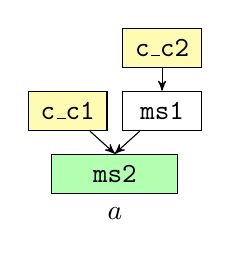
\begin{tikzpicture}[->,>=stealth']

    \node[rectangle,
          draw,
          fill = green!30,
          minimum width = 1.6cm, 
          minimum height = 0.5cm
          ] (ms4) at (0,0) {};
    \node[] at (ms4.center) {\texttt{ms2}};

    \node[rectangle,
        draw,
        minimum width = 1cm, 
        minimum height = 0.5cm
        ] (ms2) at (.6,.8) {};
    \node[] at (ms2.center) {\texttt{ms1}};


    \node[rectangle,
        draw,
        fill = yellow!30,
        minimum width = 1cm, 
        minimum height = 0.5cm
        ] (sys) at (-.6,.8) {};
    \node[] at (sys.center) {\texttt{c\_c1}};

    \node[rectangle,
        draw,
        fill = yellow!30,
        minimum width = 1cm, 
        minimum height = 0.5cm
        ] (vc) at (.6,1.6) {};
    \node[] at (vc.center) {\texttt{c\_c2}};

    \node[rectangle,
        minimum width = 1cm, 
        minimum height = 0.5cm
        ] (label) at (0,-.5) {};
    \node[] at (label.center) {$a$};


    \path[every node/.style={font=\sffamily\small}]
    %host1 path
    (vc) edge [] node [right] {} (ms2.north) 
    (sys) edge [] node [right] {} (ms4.north)
    (ms2) edge [] node [right] {} (ms4.north) ;


\end{tikzpicture} & 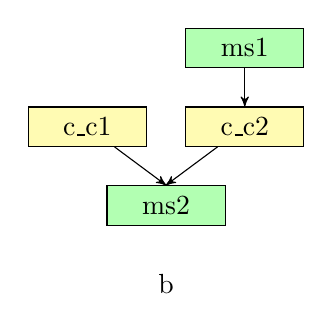
\begin{tikzpicture}[->,>=stealth']

    \node[rectangle,
          draw,
          fill = green!30,
          minimum width = 1.5cm, 
          minimum height = 0.5cm
          ] (ms4) at (0,0) {};
    \node[] at (ms4.center) {ms2};

    \node[rectangle,
        draw,
        fill = green!30,
        minimum width = 1.5cm, 
        minimum height = 0.5cm
        ] (ms2) at (1,2) {};
    \node[] at (ms2.center) {ms1};


    \node[rectangle,
        draw,
        fill = yellow!30,
        minimum width = 1.5cm, 
        minimum height = 0.5cm
        ] (sys) at (-1,1) {};
    \node[] at (sys.center) {c\_c1};

    \node[rectangle,
        draw,
        fill = yellow!30,
        minimum width = 1.5cm, 
        minimum height = 0.5cm
        ] (vc) at (1,1) {};
    \node[] at (vc.center) {c\_c2};

    \node[rectangle,
        minimum width = 1cm, 
        minimum height = 0.5cm
        ] (label) at (0,-1) {};
    \node[] at (label.center) {b};


    \path[every node/.style={font=\sffamily\small}]
    %host1 path
    (vc) edge [] node [right] {} (ms4.north) 
    (sys) edge [] node [right] {} (ms4.north)
    (ms2) edge [] node [right] {} (vc.north) ;


\end{tikzpicture} & 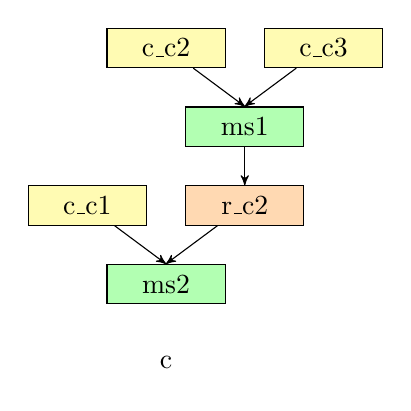
\begin{tikzpicture}[->,>=stealth']

    \node[rectangle,
          draw,
          fill = green!30,
          minimum width = 1.5cm, 
          minimum height = 0.5cm
          ] (ms4) at (0,-1) {};
    \node[] at (ms4.center) {ms2};

    \node[rectangle,
        draw,
        fill = green!30,
        minimum width = 1.5cm, 
        minimum height = 0.5cm
        ] (ms2) at (1,1) {};
    \node[] at (ms2.center) {ms1};


    \node[rectangle,
        draw,
        fill = yellow!30,
        minimum width = 1.5cm, 
        minimum height = 0.5cm
        ] (sys) at (-1,0) {};
    \node[] at (sys.center) {c\_c1};

    \node[rectangle,
        draw,
        fill = yellow!30,
        minimum width = 1.5cm, 
        minimum height = 0.5cm
        ] (c2) at (0,2) {};
    \node[] at (c2.center) {c\_c2};

    \node[rectangle,
        draw,
        fill = yellow!30,
        minimum width = 1.5cm, 
        minimum height = 0.5cm
        ] (vc) at (2,2) {};
    \node[] at (vc.center) {c\_c3};

    \node[rectangle,
        draw,
        fill = orange!30,
        minimum width = 1.5cm, 
        minimum height = 0.5cm
        ] (r1) at (1,0) {};
    \node[] at (r1.center) {r\_c2};

    \node[rectangle,
        minimum width = 1cm, 
        minimum height = 0.5cm
        ] (label) at (0,-2) {};
    \node[] at (label.center) {c};


    \path[every node/.style={font=\sffamily\small}]
    %host1 path
    (r1) edge [] node [right] {} (ms4.north) 
    (c2) edge [] node [right] {} (ms2.north) 
    (vc) edge [] node [right] {} (ms2.north) 
    (sys) edge [] node [right] {} (ms4.north)
    (ms2) edge [] node [right] {} (r1.north) ;


\end{tikzpicture} 
%     \end{tabular}
%     \caption[Example Chase Models]{Example Chase models}
%     \label{fig:chase-ex}
% \end{figure}


%The Chase generated attack graphs presented in Figure \ref{fig:chase-ex} reveal hypothetical corruption and repair events, providing essential insights for developing an adversary-constrained protocol ordering. In Figure \ref{fig:chase-ex}.a, corruption events \emph{c\_c1} and \emph{c\_c2} occur before any measurement events, implying that the adversary's actions are not time-constrained. They must simply be completed before the measurement begins. This is perhaps advantageous to an adversary because they are not forced to operate in a timely manner. In Figure \ref{fig:chase-ex}.b, the adversary is confined to perform a recent corruption as their efforts must be completed between measurement actions. This is more challenging for an adversary because they must work in an unknown time window. In Figure \ref{fig:chase-ex}.c, an adversary must perform three corruption events and one time-constrained repair event. This requires the adversary to exert far more effort to perform a successful attack as actionable events have increased. Upon analyzing all three graphs, it becomes apparent that Figure \ref{fig:chase-ex}.a presents the easiest attack, given the absence of time-constrained events and the minimal number of actions required by the adversary. Because of this, we assume an adversary would likely perform the attacks found in graph a to deceive a relying party. These attacks graphs are all generated by one protocol, yet when comparing this protocol to others, we seek to find a protocol where the easiest attacks (i.e. those performed in graph a) are made more difficult thus increasing adversary constraint.

%% END MOVE




\section{Overview}

% protocol -> set of attack graphs 
% need to talk about how we put it all together 
We introduce a Coq-based, formally-verified mathematical model to order attestation protocols by the difficulty required by an active adversary to attack the protocol. This ordering methodology compares two distinct Copland protocols by comparing their sets of Chase-generated attack graphs. From the graphs, we reason over a protocol's hypothesized corruption and repair events, introducing additional definitions and orderings for adversary event comparisons. These event comparisons are foundational for our adversary-constrained protocol ordering, ultimately allowing us to link preorder and equivalence relations to Copland phrases.

\begin{figure}[hbtp]
    \centering
    \captionsetup{justification=centering,margin=1cm}
    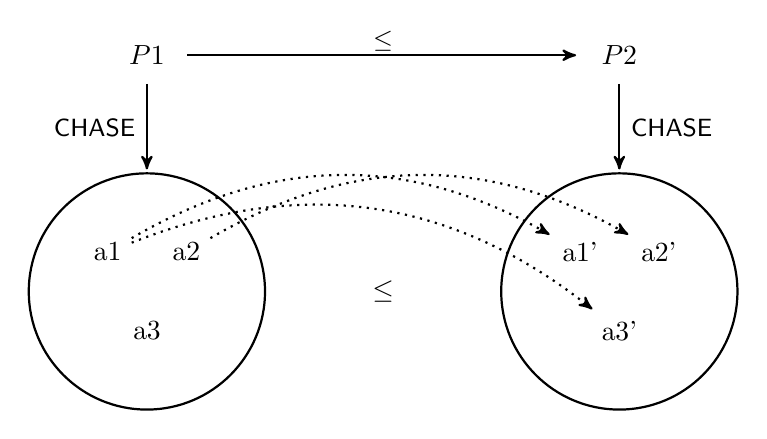
\begin{tikzpicture}[>=stealth',shorten >=1pt,auto,node distance=2.0cm,
    thick,main node/.style={rectangle,%%fill=blue!20,draw,
      font=\sffamily,minimum height=7mm,minimum width=10mm}, 
      roundnode/.style={circle, draw=black, minimum size=3cm},]
  
    \node[main node] (Phrase) {$P1$};
    %\node[main node] (ChaseP) [below of=Request] {$\langle P\rangle $};
    
    \node[main node] (Phrase') [node distance=6.0cm, right of=Phrase] {$P2$};
    % \node[main node] (ChaseP') [node distance=6.0cm, right of=Proposal] {$\langle P'\rangle$};
      
    \node[roundnode] (ChaseP) [node distance=3.0cm, below of=Phrase] {};
    \node[roundnode] (ChaseP') [node distance=6.0cm, right of=ChaseP] {};

    \node[] (a1) at (-.5,-2.5) {a1};
    \node[] (a2) at (0.5,-2.5) {a2};
    \node[] (a3) at (0,-3.5) {a3};

    \node[] (a1') at (5.5,-2.5) {a1'};
    \node[] (a2') at (6.5,-2.5) {a2'};
    \node[] (a3') at (6,-3.5) {a3'};
    %\node[] (a4') at (6.5,-3.5) {a4'};

    \node[] (ord) at (3,-3) {$\leq$};

  
    \path[every node/.style={font=\sffamily\small, fill=white,inner sep=1pt}, ->]
      (Phrase) edge node [] {$\leq$} (Phrase')
      (Phrase) edge node[left=1mm] {CHASE} (ChaseP)
      %(ChaseP) edge [dashed] node[below=1mm] {Ordering} (ChaseP')
      (Phrase') edge node[right=1mm] {CHASE} (ChaseP')
      % (a1) edge [dashed] node {} (a1')
      ;

      \draw[dotted, inner sep=0pt, ->]
        (a1) to[bend left] (a1');
      \draw[dotted, inner sep=0pt, ->]
        (a2) to[bend left] (a2');
      \draw[dotted, inner sep=0pt, ->]  
        (a1) to[bend left] (a3');
  \end{tikzpicture}
    \caption[Protocol ordering abstraction]{Diagram representing protocol ordering methodology. \\ Dashed lines represent ordering relation for individual graphs holds. }
    \label{fig:protocol-org-fig}
\end{figure}

Abstractly this analysis can be visualized in Figure \ref{fig:protocol-org-fig} where solid lines represent tangible actions and dashed lines represent reasoning. Say we aim to compare two protocols $P1$ and $P2$ where we wish to determine if the change from $P1$ to $P2$ makes the protocol more difficult to attack. Recall that more difficult to attack means more difficult for an active adversary to corrupt a system while evading detection at the final measurement event of the attestation. To ascertain the relationship between the two protocols, we first run Chase to generate the set of attack graphs $\{ a^1_1, a^1_2, a^1_3\}$ for $P1$ and the set of attack graphs for $\{a^2_1, a^2_2, a^2_3\}$ for $P2$. We then compare the Chase-generated attack graphs individually, discovering ordering relations between $a^1_1$ and $a^2_1$, $a^1_2$ and $a^2_2$, and $a^1_1$ and $a^2_3$ as represented by the dotted lines. Here, the arrow points from an attack to one that is at least as difficult to perform. Next, looking at the sets of attack graphs, we can see that every attack graph in $P2$ has a graph in $P1$ that is equal or easier to perform. Assuming an adversary would always perform the easiest attack to thwart an appraiser, we conclude that $P2$ is at least as difficult to attack as $P1$ and thus involves at least as much adversary effort as $P1$. This logic is linked to the protocols to define $ P1 \leq P2$.  

Following our workflow, we introduce four mutually inclusive relationships for an adversary-constrained protocol ordering where $=$ is an equivalence relation and $\le$ and $\ge$ are a preorder over Copland protocols. These four relations are enumerated below:

% \begin{center}
% \begin{enumerate}
%     \squash
% \item P1 = P2
% \item P1 $\le$ P2 
% \item P1 $\ge$ P2 
% \item Incomparable
% \end{enumerate}
% \end{center}
\vspace*{-10mm}

\begin{align*}
1. & P1 = P2 \\
2. & P1 \le P2 \\
3. & P1 \ge P2 \\
4. & \text{Incomparable}
\end{align*}

\noindent We choose to define the ordering in this way for a few reasons. First, we refrain from introducing four mutually exclusive relationships, finding this would result in an increase of incomparable protocols. As such, under this ordering, it is impossible to conclude that one protocol is strictly better than another protocol. We could define the relations using the irreflexive kernel (deriving a strictly less than operator from the satisfaction of both less than and not equal conditions). However, we found this was not appropriate because the strictly less than would introduce some arbitrary ordering on corruption or repair events where there should not be one.  

%% why we consider these four relations 
%% consider because they are more meaningful... could've considered the 4 mutually exclusive relations but we choose to do the overlapping... we do overlapping so less things are incomparable
%% describe why we don't conclude that sets are strictly better 
%% irreflexive kernel not an appropriate way to determine strictly better because 
%% - here you have <= and not = so you have < 
%% - if we do take the irr kernel as a relation then it puts some arbitrary ordering on corruption events where there shouldn't be one  

These four mutually inclusive relationships serve as foundational categories for adversary-constrained protocol ordering. While the ordering may appear intuitive, mathematically modeling the Chase output and subsequently comparing attacks graphs through Coq-based mechanized proofs is challenging. Our results overcome this challenge, verifying the four relationships over sets of attack graphs does provably demonstrate the properties of equivalence and preorder relations. By completing proofs over these relations, we formally define this relationship, verifying one protocol is at least as good as another because it requires at least as many adversary actions to generate seemingly trustworthy evidence. The following sections describe the process of introducing and verifying an adversary-constrained ordering between two Copland protocols. 

Under our methodology, an ordering relation between two Copland protocol can be obtained by completing the following workflow:

\begin{enumerate}
    \squash
    \item Obtain Chase output for each protocol and formally model generated attack graphs
    \item Compare individual Chase-generated attack graphs
    \item Leverage individual order to obtain ordering relation over the sets of attack graphs
    \item Link set ordering decision to obtain protocol order
\end{enumerate}

\noindent The process begins by subjecting two distinct Copland protocols to the Chase model finder to generate all possible attack graphs and then modeling the attack graphs formally in the Coq environment. Within the environment, the graphs are individually compared to determine if and how they are related. More specifically, we introduce and prove a strict partial order and an equivalence relation for comparing individual attack graphs. We leverage the ordering to then introduce the four aforementioned relationships ($=$, $\leq$, $\geq$, incomparable) over sets of attack graphs, proving equivalence and preorder relations satisfy respective properties. Once the set ordering decision is made, it is then propagated to the corresponding Copland protocols to realize protocol order. 

In the following sections, definitions and proofs pertaining to the ordering relations are stated. Here, mathematical proofs are completed manually, but mechanized versions are completed in Coq and can be found at \url{git@github.com:ku-sldg/protocol_ordering.git}. For additional accessibility, important Coq definitions and proof outlines are presented in Appendix \ref{appendix:order}.

%The first step towards this ordering is using Chase to generate individual attack graphs and subsequently comparing the relation between the individual attack graphs. We find that an individual attack graph may be either strictly less than or equal to comparable attack graph. If one of those relations hold,  Throughout the remainder of this work, we prove that the four relationships over sets of attack graphs does exhibit the properties of equivalence and preorder relations thereby formally introducing this relationship.

\section{Formalized Chase Output}

This protocol ordering scheme relies on a formal model of the Chase generated attack graphs. These graphs are similar to directed graphs which contain nodes, edges, and a labeling function. 

\begin{definition}[Directed graph]
    A directed, labeled, acyclic graph is a tuple $ G = (N, E, \ell)$ where $N$ is a finite set of nodes, $E$ is a finite set of edges represented as an edge relation $( N \times N)$, and $\ell$ is a node labeling function $\ell : N \rightarrow L$. 
\end{definition}

%% We enrich the definition of directed graphs to define attack graphs to ensure the definition better aligns with the Chase output. 
From directed graphs, the definition must be slightly enhanced to accurately capture the Chase output. Looking at Figure \ref{fig:chase-ex}, one can see that each Chase graph consists of a set of states, a relationship mapping state to state (i.e. an edge relation), and a state label disclosing the type of event -- measurement, corruption, or repair. This very closely mirrors the definition of directed graph except, in the actual Chase output, the states are labeled rather than the steps. We maintain this distinction, abstractly reasoning about corruption and repair events as adversary events, with the formal definition of an attack graph below. 

\begin{definition}[Attack Graph]
    An attack graph is a directed graph where $N$ is a set of states, $E$ are the edges representing steps between states, and $\ell$ is a labeling function from state to measurement or adversary event. 
\end{definition}

\noindent To aid in the readers understanding, we present the Coq definition for attack graphs in Figure \ref{fig:coq-graph}. This formal representation explicitly denotes the labeling mechanism for states in the attack graph as measurement event or adversary (corruption or repair) event. 

% \begin{figure}
% \begin{minted}[xleftmargin=20pt,linenos]{Coq}
%  Record attackgraph (measurement adversary : Type) : Type := 
% {   state : Type ;
%     steps : list (state * state) ;
%     label : state -> measurement + adversary }.
% \end{minted}
% \caption[]{Coq attack graph structure}
% \label{fig:coq-graph}
% \end{figure} 

When comparing two individual attack graphs, we restrict our reasoning to only events that concern an active adversary. That is, it is possible that graphs contain measurement events occurring sequentially and therfore do not impact the adversary. We found these measurements introduce unnecessary individual attack graph comparisons, negatively impacting the overall ordering decision. To refrain from considering these sequential measurements, we introduce the idea of attack graph normalization, as formally defined below. Normalization reduces any sequence of measurement events found in the attack graph to only the final measurement event in the chain. This results in attack graphs that only contain the events concerning the adversary. 

\begin{definition}[Attack Graph Normalization]
    An attack graph is in its \emph{normal form} or \emph{reduced form} when any sequence of consecutive measurement events is reduced to only the final measurement event in the chain. 
\end{definition}

\begin{figure}[htbp]
    \centering 
    \begin{tabular}{c c}
        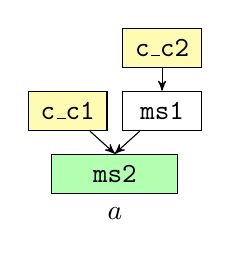
\begin{tikzpicture}[->,>=stealth']

    \node[rectangle,
          draw,
          fill = green!30,
          minimum width = 1.6cm, 
          minimum height = 0.5cm
          ] (ms4) at (0,0) {};
    \node[] at (ms4.center) {\texttt{ms2}};

    \node[rectangle,
        draw,
        minimum width = 1cm, 
        minimum height = 0.5cm
        ] (ms2) at (.6,.8) {};
    \node[] at (ms2.center) {\texttt{ms1}};


    \node[rectangle,
        draw,
        fill = yellow!30,
        minimum width = 1cm, 
        minimum height = 0.5cm
        ] (sys) at (-.6,.8) {};
    \node[] at (sys.center) {\texttt{c\_c1}};

    \node[rectangle,
        draw,
        fill = yellow!30,
        minimum width = 1cm, 
        minimum height = 0.5cm
        ] (vc) at (.6,1.6) {};
    \node[] at (vc.center) {\texttt{c\_c2}};

    \node[rectangle,
        minimum width = 1cm, 
        minimum height = 0.5cm
        ] (label) at (0,-.5) {};
    \node[] at (label.center) {$a$};


    \path[every node/.style={font=\sffamily\small}]
    %host1 path
    (vc) edge [] node [right] {} (ms2.north) 
    (sys) edge [] node [right] {} (ms4.north)
    (ms2) edge [] node [right] {} (ms4.north) ;


\end{tikzpicture} & \input{examples/general-example/four.tex} 
    \end{tabular}
    \captionsetup{justification=centering,margin=1cm}
    \caption[Example of attack graph normalization]{An example of attack graph normalization. \\ Arrow denotes from original form to normalized form.}
    \label{fig:reduce-ex}
\end{figure}
\noindent To demonstrate attack graph normalization, consider the example presented in Figure \ref{fig:reduce-ex} where graph a, taken from Figure \ref{fig:chase-ex}.a, is normalized to Figure \ref{fig:reduce-ex}.a'. When applying normalization, the sequential measurement events \texttt{ms1} and \texttt{ms2} are reduced to only the final measurement event \texttt{ms2}. 


Attack graph normalization is performed in Coq with the relational definition of \texttt{reducer} as seen in Figure \ref{fig:coq-reducer}. \texttt{reducer} is not defined as a recursive fixpoint because, to Coq's termination checker, it is not obvious the list of steps is getting smaller. Instead, \texttt{reducer} is defined as an inductive proposition to express that the graphs eventually reduce. The two constructors of \texttt{reducer} rely on a call to \texttt{reduce1}, a function that performs one reduction step. In the \texttt{reduce\_done} constructor, a call to \texttt{reduce1} returns its input revealing the graph cannot be further reduced. In the \texttt{reduce\_more} constructor, \texttt{reduce1} does not return its input and the \texttt{reducer} call is repeated.

% \begin{figure}[ht]
%     \begin{minted}[xleftmargin=20pt,linenos]{Coq}
% Inductive reducer : (G.(steps)) -> (G.(steps)) -> Prop :=
% | reduce_done : forall x, reduce1 x = x -> 
%                           reducer x x
% | reduce_more : forall x y, reduce1 x <> x -> 
%                             reducer (reduce1 x) y ->
%                             reducer x y.  
%   \end{minted}
%   \caption[]{Coq \texttt{reducer} definition to normalize attack graphs}
%   \label{fig:coq-reducer}
%   \end{figure} 

To ensure \texttt{reducer} behaves as expected, we prove that it is deterministic. Given the same inputs, the reducer will always traverse through the same states, producing equivalent outputs. This theorem and subsequent proof are described below.

\begin{theorem}[Reducer Deterministic]
    For any lists of steps $x$, $y$, and $z$ in an attack graph $G$, if $x$ reduces to $y$ and $x$ reduces to $z$, then $y=z$.
\end{theorem}
\begin{proof}
Let $x$, $y$, and $z$ be arbitrary lists of steps in an attack graph $G$. Suppose $x$ reduces to $y$ and $x$ reduces to $z$. We aim to show that $y = z$. We proceed by induction on the reduction steps

\begin{itemize}
    \squash
    \item In the base case, if $x$ reduces to $y$ via the \texttt{reduce\_done} rule, it means \texttt{reduce1}$(x) = x$. Since $x$ reduces to $z$, \texttt{reduce1}$(x)$  also reduces to $z$.
    \item In the inductive case, If $x$ reduces to $y$ via the \texttt{reduce\_more} rule, it means \texttt{reduce1}$(x) \neq x$. Let $x'$ be the result of applying \texttt{reduce1} to $x$, i.e., \texttt{reduce1}$(x)= x'$. Then, by the induction hypothesis, $y' = z'$, where $y'$ is the result of applying \texttt{reduce1} to $y$ and $z'$ is the result of applying \texttt{reduce1} to $z$. Since $y' = z'$, and $x'$ reduces to $y'$ and $x'$ reduces to $z'$ (by \texttt{reduce\_more}), we can apply the inductive hypothesis to conclude that $y' = z'$. Therefore, $y = z$ since $y' = z'$ and $y$ reduces to $y'$ and $z$ reduces to $z'$.
\end{itemize}

By induction, we have shown that if $x$ reduces to $y$ and $x$ reduces to $z$, then $y = z$.
\end{proof}

\noindent This proves that \texttt{reducer} behaves as expected and can be leveraged to normalize attack graphs. For the remainder of this Chapter, unless otherwise noted, we assume all Chase-generated attack graphs are in their normalized form, therefore only contain events that concern an adversary.

\section{Ordering}

Our main contribution lies in introducing an adversary-constrained protocol ordering through analysis of Chase-generated attack graphs. Formally defined attack graphs introduce necessary structures for reasoning. Yet, we still must institute operations to compare attack difficulty. In the following section, we establish definitions to compare adversary events and utilize these definitions to reason over attack graphs individually. Specifically, we prove a strict partial order and equivalence relations for comparing individual attack graphs. We then leverage these relations, and additional definitions, to introduce equivalence and preorder relations over sets of attack graphs. Finally, we link the ordering decision over sets of attack graphs to the corresponding Copland protocols to introduce a formally-verified adversary-constrained protocol order. Formal definitions and mathematical proofs are described in the following section. Mechanized proofs are available in Coq at \url{git@github.com:ku-sldg/protocol_ordering.git}

\subsection*{Ordering Individual Attack Graphs}

To compare individual Chase-generated attack graphs, we introduce additional definitions to determine when one attack graph requires strictly more effort or equivalent effort to attack. Central to this comparison is the formal definition of adversary actions that may be present within an attack graph. That is, Chase generated attack graphs contain measurement and adversary events. Measurement events are self-explanatory. Adversary events include corruption and repair events and are formally defined below.

%ultimately defining and proving strict partial order ($<$) and equality ($=$) relations hold. To do this, we must introduce additional definitions for determining when one attack graph is strictly better than another attack graph. Attack graphs are comprised of adversary events and measurement events. While measurement events are intuitive, adversary events must be formally defined, as presented below. 

\begin{definition}[Adversary Event]
    An adversary event is an action performed by an adversary to change the behavior of a component in a target system. Within the Chase output, adversary events are classified as  corruption or repair events. 
\end{definition}

\noindent To reason over individual attack graphs, we must consider all adversary actions present in the graph. For each graph, we therefore study the output to derive a set containing all present, abstractly denoted, adversary events. We then use these sets to compare adversary actions between individual graphs. For set comparisons, we adopt the idea of adversary event subsets and adversary event proper subsets, as formally defined below. 

\begin{definition}[Adversary Event (Proper) Subset]
    The set of adversary events of a graph a1 is an adversary event (proper) subset of the set of adversary events of a graph a2 if and only if all adversary events of a1 are contained in a2 (and a2 contains at least one adversary event not in a1).
 \end{definition}
 %-- $a2 \subset a1$ ($a2 \subseteq a1 $) -- 

As previously alluded to, time constraints escalate difficulty. That is, we assume the difficulty of an attack is increased if an adversary must complete it between measurement events. To realize this distinction, we classify time-constrained adversary events formally below:  

\begin{definition}[Time-Constrained Adversary Event]
    A time-constrained adversary event is one where the attacker must perform the corruption or repair of a component in between measurement events thus limiting the time they have to complete the action.  
\end{definition}

\noindent For comparing time-constrained adversary events between individual attack graphs, we again define time-constrained adversary event subsets and time-constrained adversary event proper subsets.
 
 \begin{definition}[Time-Constrained Adversary Event (Proper) Subset]   
    The set of time-constrained adversary events of a graph a1 is a time-constrained adversary event (proper) subset of the set of time-constrained adversary events of a graph a2 if and only if all time-constrained adversary events of a1 are contained in a2 (and a2 contains at least one time-constrained adversary event not in a1).
 \end{definition}

Adversary event (proper) subsets and time-constrained adversary event (proper) subsets serve as the basis for comparing events within individual attack graphs. It is from these definitions that we are able to subsequently model and prove equivalence and strict partial order relations over individual Chase-generated graphs. 
%The ordering conditions over individual attack graphs are explained in further detail in the following subsections. 

\subsubsection*{Individual Attack Graph Equivalence}

We say two individual attack graphs are equivalent if the graphs are semantically equivalent. Defining equivalence in this way ensures graphs which have the same adversary events in the same order are indeed equivalent, regardless of inconsequential measurement events. It is easy to visualize the case where two attack graphs that are structurally equivalent have the exact same set of states, steps, and labels and are therefore equal. However, consider the graphs in Figure \ref{fig:reduce-ex}. We wish to say \emph{a'} is equivalent to \emph{a} because both graphs have the same set of adversary events. A natural model to compare the semantics of attack graphs begins with the definition of homomorphism.

%With this notion of semantic equivalence defined as a bidirectional homomorphism, we can prove this is true.  

%\footnote[1]{From this point on, we use equivalence ($=$) and bidirectional homomorphism interchangeably.}. 

%have the same states, steps, and labels. There is one exception, however, which is that we are not concerned with measurement events which place no additional burden on the adversary.  While we care about the final measurement event being the same, equivalence for an adversary ordering does not concern unconstrained measurement events. This distinction allows us to compare protocols which have the same final measurement but potentially different prepended measurements. Because of this condition, we introduce a semantic equivalence rather than a 


\begin{definition}[Homomorphism]
    A labeled (graph) homomorphism $\eta : G \to H$ between graphs \\ $G = (N_G, E_G, l_G)$ and $H = (N_H, E_H, l_H)$ is a function $\eta : N_G \to N_H$ on the nodes such that for every edge $(n_1, n_2) \in E_G$, $(\eta(n_1), \eta(n_2)) \in E_H$, and for every node $n \in N_G$, $l_G(n) = l_H(n)$.  \cite{Rowe:2021:OnOrdering}
\end{definition}

A homomorphism is a relation between two graphs, $G$ and $H$, where $G$ and $H$ are homomorphic if there exists some function mapping the nodes of $G$ to the nodes of $H$ such that all edges in $G$ have a corresponding edge in $H$ and all labeled nodes in $G$ have related labeled nodes in $H$. To prove two graphs are homomorphic, one must obtain any function that satisfies the homomorphism relation. To prove a homomorphism does not exist, one must prove no functions are satisfactory. 

Homomorphisms provide one-way comparisons, yet equality must compare individual attack graphs bidirectionally. A seemingly natural result for bidirectional comparison from a homomorphism is an isomorphism (bijective homomorphism). However, in the context of attack graphs, the homomorphism relation does not necessarily have a one-to-one correspondence. Because of this, we cannot use an isomorphism for equality. Instead, we propose that an equality relation between individual attack graphs is a bidirectional homomorphism or the existence of a labeled attack graph homomorphism in both directions. The formal definition is presented below.

\begin{definition}[Bidirectional Homomorphism (Attack Graph Equivalence)]
    We say two attack graphs $G$ and $H$ are equivalent if there exists a  homomorphism $\eta : N_G \to N_H$ from $G$ to $H$ and a homomorphism $\phi : N_H \to N_G$ from $H$ to $G$.
\end{definition}

Proving a bidirectional homomorphism is an equivalence relation requires proofs of reflexivity, symmetry, and transitivity over the bidirectional homomorphism relation. We complete these proofs in Coq and present important facets of the mechanized code in Appendix \ref{appendix:order}. In the following text, a mathematical representation of the theorems and proofs is outlined beginning with a proof of reflexivity followed by proofs of symmetry and transitivity. In these proofs, we use equivalence and bidirectional homomorphism interchangeably.

\begin{theorem}[Reflexivity of Attack Graph Equivalence]
    Let $g1$ be an attack graph. It is true that $g1$ is equivalent to $g1$.
\end{theorem}
\begin{proof}
    An attack graph is homomorphic to itself via $\eta : g1 \to g1$. This proves reflexivity. 
\end{proof}

\begin{theorem}[Symmetry of Attack Graph Equivalence]
    Let $g1$ and $g2$ be attack graphs. If $g1$ is equivalent to $g2$ then $g2$ is equivalent to $g1$. 
\end{theorem}
\begin{proof}
    If $g1$ is homomorphic to $g2$ then there exists a function, $\eta : g1 \to g2$. Because an equivalence is defined as a bidirectional homomorphism, there exists some $\eta^{-1} : g2 \to g1$. Thus, $g2$ is homomorphic to $g1$ via $\eta^{-1}$. This proves the bidirectional homomorphism is symmetric. 
\end{proof}

\begin{theorem}[Transitivity of Attack Graph Equivalence]
    Let $g1$, $g2$, and $g3$ be attack graphs. Then if $g1$ is equivalent to $g2$ and $g2$ is equivalent to $g3$ then it is true by transitivity that $g1$ is equivalent to $g3$.   
\end{theorem}
\begin{proof}
    If $g1$ is homomorphic to $g2$ then there exists a function, $\phi : g1 \to g2$. If $g2$ is homomorphic to $g3$ then there exists a function, $\theta : g2 \to g3$. Because an equivalence is defined as a bidirectional homomorphism, there exists some $\phi^{-1} : g2 \to g1$ and $\theta^{-1} : g3 \to g2$. By functional composition, $g3$ is equivalent to $g1$ via $\theta^{-1} (\phi^{-1}).$
\end{proof}

\noindent With these three completed proofs, we obtain a formally-verified equality relation over individual attack graphs allowing us to provably determine if two graphs are semantically equivalent.

\subsubsection*{Individual Attack Graph Strict Partial Order}

A strict partial order over individual attack graphs reveals that one attack graph is strictly better than another if it increases the burden of an attacker. To formally define the concept of increasing adversary constraint, we analyzed many Chase-generated attack graphs to ground our logic in concrete examples. By studying patterns in the graphs, it is evident that an adversary could be confined under two distinct conditions. That is, an attack has increased difficulty if it requires more adversary events or more time-constrained adversary events. More formally stated, if an attack graph $a1$ is an adversary event proper subset of $a2$ then we would conclude $a2$ is strictly better than $a1$ because more corruption events requires more work on the adversary's behalf. Secondly, if an attack graph $a1$ is a time-constrained adversary event proper subset of $a2$ then we would conclude $a2$ is strictly better than $a1$ because a time-constrained corruption event requires more work. These ideas are captured with the formal definition for strict partial order below.

\begin{definition}[Strict Partial Order $<$]
    An attack graph $a1$ is strictly less than an attack graph $a2$ ($a1 < a2$) if one of the following hold: 
\begin{enumerate}
    \squash
    \item $a1$ is an adversary event subset and $a1$ is a time-constrained adversary event proper subset
    \item $a1$ is a time-constrained adversary event subset and $a1$ is an adversary event proper subset
\end{enumerate}
\end{definition}

This definition of strict partial order ($a1 < a2$) over individual attack graphs implies that graphs can only be compared if $a1$ is both an adversary event subset and time-constrained adversary event subset of $a2$. Additionally, $a1$ must either be an adversary event proper subset or time-constrained adversary proper subset of $a2$ to produce a strict partial order. To formally verify this is indeed a strict partial order, we prove the relation is irreflexive, asymmetric, and transitive using $<$ to imply strict partial order. We begin by proving irreflexivity below.

%In summary, this ordering over individual attack graphs relies upon the previously defined subset relations to determine if an attack graph better confines an adversary. 

%We prove that this relation is irreflexive, asymmetric, and transitive to ensure it is indeed a strict partial order. We complete these proofs by hand below, utilizing strictly less than and the $<$ operator interchangeably, and have completed mechanized versions in Coq.

\begin{theorem}[Irreflexivity of Strict Partial Order]
    Let $g1$ be an attack graph. It is not true that $g1$ is strictly less than itself.
\end{theorem}
\begin{proof}
    Let $g1$ be an arbitrary attack graph generated by Chase. Proceed with a proof by contradiction. Assume that $g1 < g1$. By the definition of strict partial order, all adversary events and all time-constrained adversary events are included in the subsets of $g1$. Then either the adversary events or time-constrained adversary events of $g1$ are a proper subset of $g1$. Consider the case where the set of corruption events of $g1$ is a proper subset of the set of corruption events to $g1$. By the definition of event proper subset, we find that $g1$ is a subset of the events in $g1$ and also $g1$ is not a subset of the events in $g1$. This leads to a contradiction as the two facts cannot simultaneously be true. The case is analogous for time-constrained adversary events.  Therefore, the initial assumption must be false $g1 < g1$ implying $\neg g1 < g1$ is true. 
\end{proof}

\noindent Proving asymmetry over the strict partial order follows a similar structure to the irreflexivity proof. 

\begin{theorem}[Asymmetry of Strict Partial Order]
    Let $g1$ and $g2$ be attack graphs. If $g1$ is strictly less than $g2$ then $g2$ is not strictly less than $g1$. 
\end{theorem}
\begin{proof}
    Let $g1$ and $g2$ be arbitrary attack graph generated by Chase. Assume that $g1 < g2$. By the definition of strict partial order, both the adversary events and the time-constrained adversary events of $g1$ are included in the subset of adversary events of $g2$. Then either the time-constrained adversary events or general adversary events of $g1$ are a proper subset of the adversary events of $g2$. Consider the case where the case where the set of corruption events of $g1$ is a proper subset of the set of corruption events to $g2$. The case is analogous for time-constrained adversary events.  By the definition of event proper subset, we find that $g1$ is a subset of the events in $g2$ and also $g2$ is not a subset of the adversary events in $g1$. This proves that $\neg g2 < g1$ holds because the strict partial order $<$ is the conjunction that includes the fact that $g2$ is a subset of the adversary events of $g1$. Therefore, $g1 < g2$ provably implies $\neg g2 < g1$. 
\end{proof}

\noindent Proving transitivity of the strict partial order is more arduous than the proofs of irreflexivity and asymmetry. In the Coq-based formalism, an important lemma is necessary for completing the proof. That is, the subset relation is transitive. It follows that adversary event subset and time-constrained adversary event subset relations are transitive. With this fact, completing transitivity over the strict partial order involves proof by cases for each case of the proper subset relations.

\begin{theorem}[Transitivity of Strict Partial Order]
    Let $g1$, $g2$, and $g3$ be attack graphs. Then if $g1$ is strictly less than $g2$ and $g2$ is strictly less than $g3$ then, by transitivity, $g1$ is strictly less than $g3$. 
\end{theorem}
\begin{proof}
    Let $g1$ $g2$ and $g3$ be arbitrary attack graphs. Assume $g1$ is strictly less than $g2$ and $g2$ is strictly less than $g3$. By the definition of strict partial order, both the adversary events and the time-constrained adversary events of $g1$ are included in the set of adversary events of $g2$. Then either the time-constrained adversary events or general adversary events of $g1$ are a proper subset of the adversary events of $g2$.  By the definition of strict partial order, both the adversary events and the time-constrained adversary events of $g2$ are included in the subset of adversary events of $g3$. Then either the time-constrained adversary events or general adversary events of $g2$ are a proper subset of the adversary events of $g3$. Based on the definition of strict partial order, we then need to consider the following four cases: 
    \begin{enumerate}
        \squash
        \item If the adversary events of $g1$ are a proper subset of the adversary events of $g2$ and the adversary events of $g2$ are a proper subset of the adversary events of $g3$, then by transitivity of adversary event proper subset, we conclude the set of adversary events of $g1$ are contained in the adversary events of $g3$ 
        \item If the time-constrained adversary events of $g1$ are a proper subset time-constrained adversary events of $g2$ and the time-constrained adversary events of $g2$ are a proper subset of the time-constrained adversary events of $g3$, then by transitivity of time-constrained adversary event proper subset, we conclude the set of time-constrained adversary events of $g1$ are contained in the time-constrained adversary events of $g3$  
        \item If the adversary events of $g1$ are a proper subset of the adversary events in $g2$ and if the time-constrained adversary events of $g2$ are a proper subset of the time-constrained adversary events of $g3$, then we know the set adversary events of $g1$ are contained in the adversary events of $g3$
        \item If the time-constrained adversary events of $g1$ are a proper subset of the time-constrained adversary events in $g2$ and if the adversary events of $g2$ are a proper subset of the adversary events of $g3$, then we know the set of time-constrained adversary events of $g1$ are contained in the adversary events of $g3$
    \end{enumerate}
   In all cases, we either have that the set of adversary events of $g1$ is a subset of the set of adversary events of $g3$ or the set of the time-constrained adversary events of $g1$ is a subset of time-constrained adversary events of $g3$. Then, either the set of adversary events of $g1$ is a proper subset of the set of adversary events of $g3$ or the set of the time-constrained adversary events of $g1$ is a proper subset of time-constrained adversary events of $g3$. Therefore, $g1$ is strictly less than $g3$. 
\end{proof}

Completing proofs of irreflexivity, asymmetry, and transitivity allows us to establish a formally-defined strict partial ordering relation for comparing individual attack graphs. With this, we can realize if an individual attack graph is strictly better than another, a paramount result towards our adversary-constrained protocol ordering.

\subsection*{Ordering Sets of Attack Graphs}

The previously introduced relations of equality and strict partial order between individual attack graphs can be leveraged to compare protocols by ordering their corresponding set of Chase-generated attack graphs. Yet, before any set ordering decision can be realized, we introduce additional infrastructure to compare sets of attack graphs. We begin by recalling Rowe's definition of supports and covers below \cite{Rowe:2021:OnOrdering}:

\begin{definition}[Supports/Covers]
    Given two sets of graphs S and T and some relation over the sets R, we say that S supports T iff for every $H \in T$, there is some $G \in S$, such that $R\: G\: H$. We  say that T covers S iff for every $G \in S$ there is some $H \in T$ such that $R\: G\: H$.
\end{definition}

Supports states that, for every graph in $T$, there exists some related graph in $S$. Conversely, covers says that, for every graph in $S$, there exists a related graph in $T$.  This idea is best visualized within Figure \ref{fig:sup-cov} where we abstractly denote Copland protocols as $S$ and $T$. We assume these protocols generate the corresponding set of attack graphs $\{s1, s2 , s3 \}$ and $ \{t1, t2 ,t3\}$.

\begin{figure}[htbp]
    \centering
    \usetikzlibrary{shapes.geometric}

\begin{tikzpicture}


    \node[ellipse,
    draw = black,
    minimum width = 1.5cm, 
    minimum height = 3cm] (e) at (-4.8,0) {};

    \node[ellipse,
    draw = black,
    minimum width = 1.5cm, 
    minimum height = 3cm] (e) at (-1.8,0) {};

    \node[ellipse,
    draw = black,
    minimum width = 1.5cm, 
    minimum height = 3cm] (e) at (1.8,0) {};

    \node[ellipse,
    draw = black,
    minimum width = 1.5cm, 
    minimum height = 3cm] (e) at (4.8,0) {};


    \node[] (a1) at (-4.8,.8) {$a_1$};
    \node[] (a2) at (-4.8,0) {$a_2$};
    \node[] (a3) at (-4.8,-.8) {$a_3$};

    \node[] (a1') at (-1.8,.8) {$b_1$};
    \node[] (a2') at (-1.8,0) {$b_2$};
    \node[] (a3') at (-1.8,-.8) {$b_3$};

    \node[] (b1) at (4.8,.8) {$b_1$};
    \node[] (b2) at (4.8,0) {$b_2$};
    \node[] (b3) at (4.8,-.8) {$b_3$};

    \node[] (b1') at (1.8,.8) {$a_1$};
    \node[] (b2') at (1.8,0) {$a_2$};
    \node[] (b3') at (1.8,-.8) {$a_3$};

    \node[] (label) at (-3.3, -2.1) {$S$ supports $T$};
    \node[] (label) at (3.3, -2.1) {$T$ covers $S$};

    \node[] (label) at (-4.8, 1.9) {$S$};
    \node[] (label) at (-1.8, 1.9) {$T$};

    \node[] (label) at (1.8, 1.9) {$S$};
    \node[] (label) at (4.8, 1.9) {$T$};


      \draw[->] (a1) to (a1');
      \draw[->] (a2) to (a2');
      \draw[->] (a2) to (a3');

      \draw[->] (b1') to (b1);
      \draw[->] (b2') to (b1);
      \draw[->] (b3') to (b1);
  \end{tikzpicture}
    \captionsetup{justification=centering,margin=1cm}
    \caption[Supports and covers]{A visual representation of supports and covers. \\ Arrows represent ordering relation holds.}
    \label{fig:sup-cov}
\end{figure}

The definition of supports and covers states an arbitrary relation $R$ must hold between individual graphs found within the sets. For an adversary-constrained protocol ordering, we choose $R$ to be a disjunction of the previously defined equality and strict partial order relations. Therefore, supports and covers can be conceptualized as wrappers over individual attack graph comparisons where, in Figure \ref{fig:sup-cov}, arrows between the individual attack graphs $t1, ... ,tk$ and $s1, ... ,sk$ reveal either the equality or strict partial ordering relation holds. 

While Rowe defines both supports and covers, we only need to be concerned with supports for our adversary-constrained protocol ordering. To reliably conclude that $S$ supports $T$ or $S \leq T$, every graph in $T$ must have a related graph in $S$. If we have some graph in $T$ that does not have a related graph in $S$, then that unrelated graph could be the easiest attack and thus most likely for the adversary to perform. Because of this, if we omit even one graph in $T$ from the comparison, then we could produce a potentially ill-formed ordering. We conclude only supports can be realized to correctly state that the protocol $T$ is at least as difficult to attack as the protocol $S$. 

Rowe's \cite{Rowe:2021:OnOrdering} definition of supports must be changed to account for the aforementioned properties. Formally stated below, this enhanced definition denotes $R$ as the previously defined equality (bidirectional homomorphism) or strict partial order relations. These relations are defined over individual graphs. By using them under supports, we are able to compare sets of attack graphs. 

\begin{definition}[Supports (Attack Graph Version)]
    Given two sets of attack graphs S and T and the equality and strict partial order relation over the sets, we say that S supports T if and only if for every $H \in T$, there is some $G \in S$, such that $G$ equals $H$ or $G$ is strictly less than $H$.
\end{definition}

% \begin{lstlisting}[language=Coq]
% Definition supports' (SS TT: list (attackgraph measurement corruption)) : Prop := 
%   forall (H : (attackgraph measurement corruption)), In H TT ->
%   (exists (G : (attackgraph measurement corruption)), In G SS /\ 
%   (bidir_homo G H \/ strict_partial_order G H)).
% \end{lstlisting}

\noindent Supports is a preorder over sets of Chase-generated attack graphs. Verifying this is indeed a preorder requires proofs of reflexivity and transitivity. Mathematical versions of these proofs are completed below. Mechanized proofs are available in Coq.  

\begin{theorem}[Reflexivity of Supports]
    Let $SS$ be a set of attack graphs. It is true that $SS$ supports itself.
\end{theorem}
\begin{proof}    
    Let $SS$ be an arbitrary set of attack graphs. Let $G$ be an arbitrary graph in $SS$. By the definition of supports, $G$ is equal to or strictly less than itself. Therefore $SS$ supports itself. 
\end{proof}

\begin{theorem}[Transitivity of Supports]
    Let $SS$, $TT$, and $PP$ be sets of attack graphs. Then if $SS$ supports $TT$ and $TT$ supports $PP$ then it is true by transitivity that $SS$ supports $PP$. 
\end{theorem}
\begin{proof}
    Let $SS$, $TT$, and $PP$ be arbitrary sets of attack graphs. Assume $SS$ supports $TT$ and $TT$ supports $PP$. Let $p$ be an arbitrary graph in $PP$. Then by the assumption that $TT$ supports $PP$, there must exist some $t$ in $TT$ such that $t$ is bidirectionally homomorphic or strictly less than $p$. By the assumption that $SS$ supports $TT$, there must exist some $s$ in $SS$ such that $s$ is bidirectionally homomorphic or strictly less than $t$. Therefore, $p$ is bidirectionally homomorphic to or strictly less than $s$. We conclude that $SS$ supports $PP$
\end{proof}

\noindent Completing these proofs stipulates that supports is a preorder over sets of attack graph. We therefore proved that one set of attack graphs is at least as difficult to attack compared to another. Linking the preorder decision over sets of attack graphs to their corresponding protocols allows us to provably state that one protocol is at least as difficult to attack as another protocol. From here on, we use supports, $\leq$, and less than or equal to interchangeably. 

Recall we introduce four mutually inclusive relations. While we now have a preorder $\leq$ over sets of attack graphs, we must also introduce a verified equivalence relation to ascertain when two sets of Chase-generated attack graphs are equivalent. Set equality is defined in the same way as supports (attack graph version) sans the strictly less than relation. This formally stated as follows: 

\begin{definition}[Set Equality]
    Two sets of attack graphs $S$ and $T$ are equivalent if and only if for every $H \in T$, there is some $G \in S$, such that $G$ is bidirectionally homomorphic to $H$ and for every $G \in S$, there is some $H \in T$, such that $H$ is bidirectionally homomorphic to $G$.
\end{definition}

This definition of set equality is essentially a bidirectional version of supports with equivalence (bidirectional homomorphism) over individual graphs as $R$. We prove that set equality is indeed an equivalence relation by proving reflexivity, symmetry, and transitivity. 

\begin{theorem}[Reflexivity of Set Equivalence]
    Let $SS$ be a set of attack graphs. It is true that, by set equivalence, $SS$ is equivalent to $SS$.
\end{theorem}
\begin{proof}
    This proof is trivial.  
\end{proof}

%% TODO: better word for equivalent 
%% TODO: change wording in Coq file to reflect 

\begin{theorem}[Symmetry of Set Equivalence]
    Let $SS$ and $TT$ be sets of attack graphs. If the set $SS$ is equivalent to the set $TT$ by set equivalence then $TT$ is equivalent to $SS$. 
\end{theorem}
\begin{proof}
    Let $SS$ and $TT$ be sets of attack graphs. For any graph $H$ in $TT$, there exists a graph $G$ in $SS$ such that $G$ and $H$ are bidirectionally homomorphic. This follows from the definition of set equality. By the same logic, for every graph $G$ in $SS$, there exists a graph $H$ in $TT$ such that $G$ and $H$ are bidirectional homomorphic. Again, this follows from the definition of set equality. Since $TT$ supports $SS$ under the bidirectional homomorphism and $SS$ supports $TT$ under bidirectional homomorphism, we can conclude that $TT$ is equivalent to $SS$ 
\end{proof}

\begin{theorem}[Transitivity of Set Equivalence]
    Let $SS$, $TT$, and $PP$ be sets of attack graphs. Then if $SS$ is equivalent to $TT$ by set equivalence and $TT$ is equivalent to $PP$ by set equivalence then it is true by transitivity that $SS$ is equivalent to $PP$ by set equivalence.   
\end{theorem}

\begin{proof}
Let $SS$, $TT$, and $PP$ be arbitrary sets of graphs. Assume sets SS and TT are equivalent and sets TT adn PP are equivalent, where equivalence is supports with a bidirectional homomorphism for This implies the following conditions hold:
\begin{enumerate}
    \squash
    \item For any $s$ in $SS$, there exists a $t$ in $TT$ such that $s$ and $t$ are bidirectionally homomorphic.
    \item For any $t$ in $TT$, there exists a $s$ in $SS$ such that $s$ and $t$ are bidirectionally homomorphic.
    \item For any $t$ in $TT$, there exists a $p$ in $PP$ such that $t$ and $p$ are bidirectionally homomorphic.
    \item For any $p$ in $PP$, there exists a $t$ in $TT$ such that $t$ and $p$ are bidirectionally homomorphic.
\end{enumerate}

Again, we aim to show the set $SS$ is equivalent to $PP$ by transitivity. This means the set of graphs in $SS$ is bidirectionally homomorphic to the set of graphs in $PP$ and the set of graphs in $PP$ is bidirectionally homomorphic to the set of graphs in $SS$. 

First, prove the set of graphs in $SS$ is bidirectionally homomorphic to the set of graphs in $PP$. For a given $s$ in $SS$, apply condition 1 to find a corresponding $t$ in $TT$ such that $s$ and $t$ are bidirectionally homomorphic. Then, apply condition 3 to find a corresponding $p$ in $PP$ such that $t$ and $p$ are bidirectionally homomorphic. Combining these bidirectional homomorphisms yields an bidirectional homomorphism between $s$ and $p$.

Secondly, prove the set of graphs in $PP$ is bidirectionally homomorphic to the set of graphs in $SS$. Similar to the first case, apply condition 4 to find a corresponding $t$ in $TT$ such that $t$ and $p$ are bidirectionally homomorphic. Then, apply condition 2 to find a corresponding $s$ in $SS$ such that $s$ and $H$ are bidirectionally homomorphic. Combining these bidirectional homomorphisms yields a bidirectional homomorphism between $s$ and $p$.

Since both conditions hold, we conclude that the sets $SS$ and $PP$ are equivalent by transitivity.
\end{proof}

\noindent Completing proofs of reflexivity, symmetry, and transitivity formally introduces the set equality relation. By linking the set equality decision to the corresponding protocols that produced the set of attack graphs, we are able to find that two protocols require equal difficultly to attack. Because each graph in one set has a semantically equivalent graph in the other set, the attacks require equivalent effort in the eyes of an adversary. 

With verified equivalence and preorder relations over sets of attack graphs, we can link the ordering decision to the corresponding protocol to prove if one of the four mutually inclusive relations hold. If no ordering relation holds, the protocols are incomparable. Therefore, with the additional definitions for individual attack graph comparison and set comparison, we have formally verified the four previously defined mutually inclusive relationships hold for ordering Copland protocols. By leveraging existing tools, like the Chase model finder, we were able to successfully capture all possible attacks and adversary may launch yet go undetected. This ordering reasons over those attacks, successfully introducing a proven adversary-constrained protocol ordering. 

\section{Representative Examples}

%% talk more about irreflexive kernel 
%% reduce graphs so it is easier to read 

This research finds inspiration in real-life instances of Copland protocol analysis documented in the attestation literature \cite{Rowe:2021:OnOrdering,Coker::Principles-of-R}. Motived by the attacks explained in Section \ref{section:running-ex}, we ground our formally-verified adversary-constrained protocol ordering model in reality by reasoning about a relying party who would like to ensure a remote server (target) is free of viruses. Taken from Rowe's \cite{Rowe:2016:Confining} example presented in Figure \ref{fig:Rowe_example}, this target infrastructure for all forthcoming examples is abstractly rendered in Figure \ref{fig:ord-system}. In this system, there are two platforms $P3$ and $P4$ which depend on a hardware root of trust (rtm). Additional system dependencies within $P4$ are denoted with dashed lines.  Each platform has various measurement operations (ASPs), including a virus checking measurement $vc$ and a kernel integrity measurement $ker$. From this system, we derive possible Copland protocols and perform various manipulations in protocol structure and order. We then apply previously derived formal reasoning to determine the most adversary-constrained protocol, further establishing correctness in our model.

%various attestation scenarios where all protocols result in same final measurement event of a virus checking ASP \emph{vc} performing a measurement of the target system (i.e. server) \emph{sys}. 
% The generated evidence, without undisclosed interference from an adversary, proves the target system is free from viruses. 

\begin{figure}[htbp]
    \centering
    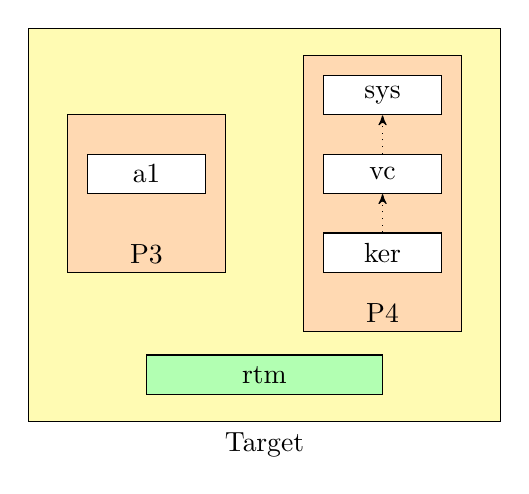
\begin{tikzpicture}[->,>=stealth']

    %\node (req) at (-6,0) {Request, *P0};

    \node[rectangle,
          draw,
          fill = yellow!30,
          minimum width = 6cm, 
          minimum height = 5cm] (r) at (0,-.4) {};
    \node[anchor=north] at (r.south) {Target};
    
    \node[rectangle,
          draw,
          fill = orange!30,
          minimum width = 2cm, 
          minimum height = 2cm] (AM) at (-1.5,0) {};
    \node[anchor=south] at (AM.south) {P3}; 

    \node[rectangle,
          draw,
          fill = white,
          minimum width = 1.5cm, 
          minimum height = 0.5cm] (ASP) at (-1.5,0.25) {};
    \node at (ASP.center) {a1};

    \node[rectangle,
          draw,
          fill = orange!30,
          minimum width = 2cm, 
          minimum height = 3.5cm] (Host2) at (1.5,0) {};
    \node[anchor=south] at (Host2.south) {P4}; 

    \node[rectangle,
          draw,
          fill = white,
          minimum width = 1.5cm, 
          minimum height = 0.5cm] (sys) at (1.5,1.25) {};
    \node at (sys.center) {sys};
    

    \node[rectangle,
    draw,
    fill = white,
    minimum width = 1.5cm, 
    minimum height = .5cm] (vc) at (1.5,0.25) {};
    \node at (vc.center) {vc};

    \node[rectangle,
    draw,
    fill = white,
    minimum width = 1.5cm, 
    minimum height = .5cm] (ker) at (1.5,-0.75) {};
    \node at (ker.center) {ker};

    \node[rectangle,
    draw,
    fill = green!30,
    minimum width = 3cm, 
    minimum height = 0.5cm] (RoTM) at (0,-2.3) {};
    \node at (RoTM.center) {rtm};



    \path[every node/.style={font=\sffamily\small}]
    %host1 path
%    (req) edge node [right] {} (r.west)
%     (ASP.east) edge[draw=red,dotted] node [left] {} (sys.west)
%     % host2 path
     (vc.north) edge [dotted] node [left] {} (sys.south)
     (ker.north) edge [dotted] node {} (vc.south);
%     (RoTM.north) edge [dotted] node {} (ker.south) ;

\end{tikzpicture}
    \captionsetup{justification=centering,margin=1cm}
    \caption[Example system for protocol ordering]{Example system for protocol ordering motivated by \cite{Rowe:2016:Confining}.\\ Dashed lines represent dependencies. }
    \label{fig:ord-system}
\end{figure}

Within the forthcoming protocol ordering examples, we maintain our initial assumption. Again, we assume that the adversary has manipulated the system and somehow allowed the resulting evidence to appear trustworthy when it is not. We also assume the root of trust (rtm) is inherently trusted and therefore cannot be attacked. We explicitly state these assumptions, and the system's dependency structure, in the Chase input files. Aside from the protocol input file, the same Chase files are used during each protocol ordering experiment. 

Extending from the framework illustrated in Figure \ref{fig:Rowe_example} and Figure \ref{fig:ord-system}, we introduce three distinct scenarios to investigate the impact of adversary constraint when manipulating measurement operations and measurement composition. In the first example, we test the effects of well-supported measurements on an attacker's difficultly of attack. In the second and third examples, we test various effects of protocol composition. Each experiment is tested under our formally defined adversary-constrained model to assign one of the four relationships.
%(presented in Appendix \ref{Appendix.Chase})

The first example hypothesizes that creating a more comprehensive protocol, one where targets and their dependencies are measured, produces more trustworthy evidence. This hypothesis was initially validated manually, relying on intuition and logical reasoning \cite{Rowe:2016:Confining}. To test this hypothesis under our formal model, we selected the following three protocols presented in Table \ref{Chase-table} where again the goal of each measurement is to ascertain if a system is free from viruses. The Copland phrase that accomplishes this is $\at{p4}{(vc\; p4\; sys)}$. This measurement is therefore the final phrase in each protocol. By maintaining the same final measurement event, we focus our investigation towards the effect of adversary constraint on protocol comprehensiveness.

\begin{table}[htbp]
    \setlength\extrarowheight{7pt}
    \centering
    \begin{tabular}{|M{4cm}|M{12cm}|N}
        \hline
        Protocol Name & Actual protocol &\\
        \hline
        sys & *target: $\at{p4}{(vc\; p4\; sys)}$  &\\ 
        %\hline
        % a1-vc-sys-seq & *target: $\at{p3}{[(a1\; p4\; vc) \braseqe\pi \at{p4}{(vc\; p4\; sys)}]}$ &\\ 
        \hline   
        ker-vc-sys-seq & *target:  $\at{p4}{[(ker\; p4\; vc)}$ \texttt{+<+} $\at{p4}{(vc\; p4\; sys)}]$ &\\ \hline 
        rtm-ker-vc-sys-seq & *target: $\at{p1}{[(rtm\; p4\; ker)}$ \texttt{+<+} $\at{p4}{[(ker\; p4\; vc)}$ \texttt{+<+} $\at{p4}{(vc\; p4\; sys)}]]$ &\\
        \hline
    \end{tabular}
    \caption[Chase Analysis with Varied Dependencies]{Sequential protocols analyzed with Chase, mimicking layered measurement style}
    \label{Chase-table}
\end{table}

When constructing this case study, we start from the simplest protocol and sequentially prepend measurement operations until reaching a root of trust, carefully crafting each protocol to mimic the system's dependencies. The first protocol, \texttt{sys}, is a measurement of the system using the virus checker. If the virus checking ASP is inadvertently corrupted, the resulting evidence will lack validity. To ensure the trustworthiness of the virus checking ASP, one may utilize one of the virus checking dependencies to measure the virus checker prior to its measurement of the system. This is achieved through the \texttt{ker-vc-sys-seq} protocol, where the kernel ASP \emph{ker} is invoked to measure the virus checker \emph{vc} before the virus checker \emph{vc} measures the system \emph{sys}. By measuring within the dependency chain, we hypothetically strengthen the resulting evidence. Taking this reasoning a step further, the protocol \texttt{rtm-ker-vc-sys-seq} includes a prepended measurement of the kernel \emph{ker}, performed by the root of trust $rtm$, prior to $ker$'s measurement of the virus checker. Because the root of trust is a trusted source, we can hypothetically further strengthen the resulting evidence. 


% \begin{figure}[hbtp]
%     \begin{center}
%         \begin{tabular}{ M{3.75cm} | M{4.75cm} | M{4.75cm} }
%                 sys & ker-vc-sys-seq & rtm-ker-vc-sys-seq \\
%                 \hline
%                 &&\\ \input{examples/sys/sys1.tex} & \input{examples/ker_vs-sys-seq/m1.tex} & \input{examples/rtm_ker-vc-sys-seq/m1.tex} \\ 
%                 m1a & m1b & m1c \\ 
%                 &&\\
%                 \begin{tikzpicture}[->,>=stealth']

    \node[rectangle,
          draw,
          fill = green!30,
          minimum width = 2cm, 
          minimum height = 0.5cm
          ] (ms4) at (0,0) {};
    \node[] at (ms4.center) {\texttt{ms4}};


    \node[rectangle,
        draw,
        fill = yellow!30,
        minimum width = 1.5cm, 
        minimum height = 0.5cm
        ] (sys) at (-1,1) {};
    \node[] at (sys.center) {\texttt{c\_sys}};

    \node[rectangle,
        draw,
        fill = yellow!30,
        minimum width = 1.5cm, 
        minimum height = 0.5cm
        ] (ker) at (1,1) {};
    \node[] at (ker.center) {\texttt{c\_ker}};

    \node[rectangle,
        minimum width = 1.5cm, 
        minimum height = 0.5cm
        ] (ms3) at (1,2) {};
    \node[] at (ms3.center) {};


    % \node[rectangle,
    %     minimum width = 1cm, 
    %     minimum height = 0.5cm
    %     ] (label) at (0,-1) {};
    % \node[] at (label.center) {m2a};


    \path[every node/.style={font=\sffamily\small}]
    %host1 path
    (vc) edge [] node [right] {} (ms4.north) 
    (sys) edge [] node [right] {} (ms4.north) ;


\end{tikzpicture} & 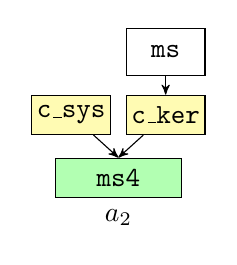
\begin{tikzpicture}[->,>=stealth']

    \node[rectangle,
          draw,
          fill = green!30,
          minimum width = 1.6cm, 
          minimum height = 0.5cm
          ] (ms4) at (0,0) {};
    \node[] at (ms4.center) {\texttt{ms4}};

    \node[rectangle,
    minimum width = 1cm, 
    minimum height = 0.5cm
    ] (lab) at (0,-.5) {};
  \node[] at (lab.center) {$a_2$};

    \node[rectangle,
        draw,
        fill = yellow!30,
        minimum width = 1cm, 
        minimum height = 0.5cm
        ] (sys) at (-.6,.8) {};
    \node[] at (sys.center) {\texttt{c\_sys}};

    \node[rectangle,
        draw,
        fill = yellow!30,
        minimum width = 1cm, 
        minimum height = 0.5cm
        ] (vc) at (.6,.8) {};
    \node[] at (vc.center) {\texttt{c\_ker}};

    \node[rectangle,
        draw,
        minimum width = 1cm, 
        minimum height = 0.6cm
        ] (ms3) at (.6,1.6) {};
    \node[] at (ms3.center) {\texttt{ms}};

%     \node[rectangle,
%     minimum width = 1cm, 
%     minimum height = 0.5cm
%     ] (label) at (0,-0.5) {};
% \node[] at (label.center) {m2b};


    \path[every node/.style={font=\sffamily\small}]
    %host1 path
    (ms3) edge [] node [right] {} (vc.north)
    (vc) edge [] node [right] {} (ms4.north) 
    (sys) edge [] node [right] {} (ms4.north) ;


\end{tikzpicture} & 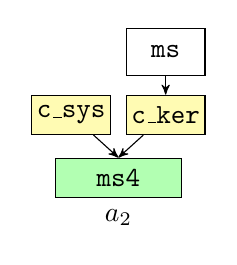
\begin{tikzpicture}[->,>=stealth']

    \node[rectangle,
          draw,
          fill = green!30,
          minimum width = 1.6cm, 
          minimum height = 0.5cm
          ] (ms4) at (0,0) {};
    \node[] at (ms4.center) {\texttt{ms4}};

    \node[rectangle,
    minimum width = 1cm, 
    minimum height = 0.5cm
    ] (lab) at (0,-.5) {};
  \node[] at (lab.center) {$a_2$};

    \node[rectangle,
        draw,
        fill = yellow!30,
        minimum width = 1cm, 
        minimum height = 0.5cm
        ] (sys) at (-.6,.8) {};
    \node[] at (sys.center) {\texttt{c\_sys}};

    \node[rectangle,
        draw,
        fill = yellow!30,
        minimum width = 1cm, 
        minimum height = 0.5cm
        ] (vc) at (.6,.8) {};
    \node[] at (vc.center) {\texttt{c\_ker}};

    \node[rectangle,
        draw,
        minimum width = 1cm, 
        minimum height = 0.6cm
        ] (ms3) at (.6,1.6) {};
    \node[] at (ms3.center) {\texttt{ms}};

%     \node[rectangle,
%     minimum width = 1cm, 
%     minimum height = 0.5cm
%     ] (label) at (0,-0.5) {};
% \node[] at (label.center) {m2b};


    \path[every node/.style={font=\sffamily\small}]
    %host1 path
    (ms3) edge [] node [right] {} (vc.north)
    (vc) edge [] node [right] {} (ms4.north) 
    (sys) edge [] node [right] {} (ms4.north) ;


\end{tikzpicture}  \\
%                 m2a & m2b & m2c \\   
%                 & \input{examples/ker_vs-sys-seq/m3.tex}  & \input{examples/rtm_ker-vc-sys-seq/m3.tex}  \\               
%                 & m3b & m3c \\ 
%                 &&\\
%                   & 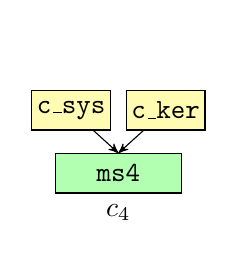
\begin{tikzpicture}[->,>=stealth']

  \node[rectangle,
        draw,
        fill = green!30,
        minimum width = 1.6cm, 
        minimum height = 0.5cm
        ] (ms4) at (0,0) {};
  \node[] at (ms4.center) {\texttt{ms4}};

  \node[rectangle,
  minimum width = 1cm, 
  minimum height = 0.5cm
  ] (lab) at (0,-.5) {};
\node[] at (lab.center) {$c_4$};

  %\node[rectangle,
  %    draw,
  %    minimum width = 1.5cm, 
  %    minimum height = 0.5cm
  %    ] (ms) at (-1,1) {};
  %\node[] at (ms.center) {ms};

  \node[rectangle,
      draw,
      fill = yellow!30,
      minimum width = 1cm, 
      minimum height = 0.5cm
      ] (ker) at (.6,.8) {};
  \node[] at (ker.center) {\texttt{c\_ker}};

  \node[rectangle,
      draw,
      fill = yellow!30,
      minimum width = 1cm, 
      minimum height = 0.5cm
      ] (sys) at (-.6,.8) {};
  \node[] at (sys.center) {\texttt{c\_sys}};

  \node[rectangle,
      minimum width = 1cm, 
      minimum height = 0.5cm
      ] (ms3) at (.6,1.6) {};
  \node[] at (ms3.center) {};

%     \node[rectangle,
%     minimum width = 1cm, 
%     minimum height = 0.5cm
%     ] (label) at (0,-0.5) {};
% \node[] at (label.center) {m3b};


  \path[every node/.style={font=\sffamily\small}]
  %host1 path
  (ker) edge [] node [right] {} (ms4.north)
  (sys) edge [] node [right] {} (ms4.north) ;
  % (ms) edge [] node [right] {} (ms4.north) ;


\end{tikzpicture} & 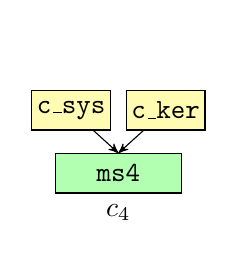
\begin{tikzpicture}[->,>=stealth']

  \node[rectangle,
        draw,
        fill = green!30,
        minimum width = 1.6cm, 
        minimum height = 0.5cm
        ] (ms4) at (0,0) {};
  \node[] at (ms4.center) {\texttt{ms4}};

  \node[rectangle,
  minimum width = 1cm, 
  minimum height = 0.5cm
  ] (lab) at (0,-.5) {};
\node[] at (lab.center) {$c_4$};

  %\node[rectangle,
  %    draw,
  %    minimum width = 1.5cm, 
  %    minimum height = 0.5cm
  %    ] (ms) at (-1,1) {};
  %\node[] at (ms.center) {ms};

  \node[rectangle,
      draw,
      fill = yellow!30,
      minimum width = 1cm, 
      minimum height = 0.5cm
      ] (ker) at (.6,.8) {};
  \node[] at (ker.center) {\texttt{c\_ker}};

  \node[rectangle,
      draw,
      fill = yellow!30,
      minimum width = 1cm, 
      minimum height = 0.5cm
      ] (sys) at (-.6,.8) {};
  \node[] at (sys.center) {\texttt{c\_sys}};

  \node[rectangle,
      minimum width = 1cm, 
      minimum height = 0.5cm
      ] (ms3) at (.6,1.6) {};
  \node[] at (ms3.center) {};

%     \node[rectangle,
%     minimum width = 1cm, 
%     minimum height = 0.5cm
%     ] (label) at (0,-0.5) {};
% \node[] at (label.center) {m3b};


  \path[every node/.style={font=\sffamily\small}]
  %host1 path
  (ker) edge [] node [right] {} (ms4.north)
  (sys) edge [] node [right] {} (ms4.north) ;
  % (ms) edge [] node [right] {} (ms4.north) ;


\end{tikzpicture}  \\
%                 & m4b & m4c \\
%                   & 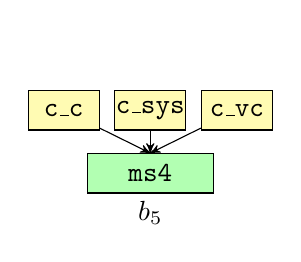
\begin{tikzpicture}[->,>=stealth']

    \node[rectangle,
          draw,
          fill = green!30,
          minimum width = 1.6cm, 
          minimum height = 0.5cm
          ] (ms4) at (0,0) {};
    \node[] at (ms4.center) {\texttt{ms4}};

    \node[rectangle,
    minimum width = 1cm, 
    minimum height = 0.5cm
    ] (lab) at (0,-.5) {};
  \node[] at (lab.center) {$b_5$};

    \node[rectangle,
        draw,
        fill = yellow!30,
        minimum width = .9cm, 
        minimum height = 0.5cm
        ] (vc) at (1.1,.8) {};
    \node[] at (vc.center) {\texttt{c\_vc}};

    \node[rectangle,
        draw,
        fill = yellow!30,
        minimum width = .9cm, 
        minimum height = 0.5cm
        ] (c) at (-1.1,.8) {};
    \node[] at (c.center) {\texttt{c\_c}};

    \node[rectangle,
        draw,
        fill = yellow!30,
        minimum width = .9cm, 
        minimum height = 0.5cm
        ] (sys) at (0,.8) {};
    \node[] at (sys.center) {\texttt{c\_sys}};

    \node[rectangle,
        minimum width = .9cm, 
        minimum height = 0.5cm
        ] (ms3) at (1.1,1.6) {};
    \node[] at (ms3.center) {};


    \path[every node/.style={font=\sffamily\small}]
    %host1 path
    (vc) edge [] node [right] {} (ms4.north)
    (c) edge [] node [right] {} (ms4.north)
    (sys) edge [] node [right] {} (ms4.north) ;
    % (ms) edge [] node [right] {} (ms4.north) ;


\end{tikzpicture} & 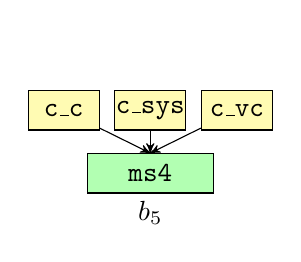
\begin{tikzpicture}[->,>=stealth']

    \node[rectangle,
          draw,
          fill = green!30,
          minimum width = 1.6cm, 
          minimum height = 0.5cm
          ] (ms4) at (0,0) {};
    \node[] at (ms4.center) {\texttt{ms4}};

    \node[rectangle,
    minimum width = 1cm, 
    minimum height = 0.5cm
    ] (lab) at (0,-.5) {};
  \node[] at (lab.center) {$b_5$};

    \node[rectangle,
        draw,
        fill = yellow!30,
        minimum width = .9cm, 
        minimum height = 0.5cm
        ] (vc) at (1.1,.8) {};
    \node[] at (vc.center) {\texttt{c\_vc}};

    \node[rectangle,
        draw,
        fill = yellow!30,
        minimum width = .9cm, 
        minimum height = 0.5cm
        ] (c) at (-1.1,.8) {};
    \node[] at (c.center) {\texttt{c\_c}};

    \node[rectangle,
        draw,
        fill = yellow!30,
        minimum width = .9cm, 
        minimum height = 0.5cm
        ] (sys) at (0,.8) {};
    \node[] at (sys.center) {\texttt{c\_sys}};

    \node[rectangle,
        minimum width = .9cm, 
        minimum height = 0.5cm
        ] (ms3) at (1.1,1.6) {};
    \node[] at (ms3.center) {};


    \path[every node/.style={font=\sffamily\small}]
    %host1 path
    (vc) edge [] node [right] {} (ms4.north)
    (c) edge [] node [right] {} (ms4.north)
    (sys) edge [] node [right] {} (ms4.north) ;
    % (ms) edge [] node [right] {} (ms4.north) ;


\end{tikzpicture} \\
%                 & m5b & m5c \\  
%             \end{tabular}
%     \end{center}
%     \caption{Attack graphs for sys, ker-vc-sys-seq, and rtm-ker-vc-sys-seq}
%     \label{fig:rtm-compare}
% \end{figure}

% \begin{figure}[hbtp]
%     \begin{center}
%         \begin{tabular}{ M{3.75cm} | M{4.75cm} | M{4.75cm} }
%                 sys & ker-vc-sys-seq & rtm-ker-vc-sys-seq \\
%                 \hline
%                 &&\\ \input{examples/sys/sys1.tex} & \input{examples/ker_vs-sys-seq_reduced/m1.tex} & \input{examples/rtm_ker-vc-sys-seq_reduced/m1.tex} \\ 
%                 m1a & m1b & m1c \\ 
%                 &&\\
%                 \begin{tikzpicture}[->,>=stealth']

    \node[rectangle,
          draw,
          fill = green!30,
          minimum width = 2cm, 
          minimum height = 0.5cm
          ] (ms4) at (0,0) {};
    \node[] at (ms4.center) {\texttt{ms4}};


    \node[rectangle,
        draw,
        fill = yellow!30,
        minimum width = 1.5cm, 
        minimum height = 0.5cm
        ] (sys) at (-1,1) {};
    \node[] at (sys.center) {\texttt{c\_sys}};

    \node[rectangle,
        draw,
        fill = yellow!30,
        minimum width = 1.5cm, 
        minimum height = 0.5cm
        ] (ker) at (1,1) {};
    \node[] at (ker.center) {\texttt{c\_ker}};

    \node[rectangle,
        minimum width = 1.5cm, 
        minimum height = 0.5cm
        ] (ms3) at (1,2) {};
    \node[] at (ms3.center) {};


    % \node[rectangle,
    %     minimum width = 1cm, 
    %     minimum height = 0.5cm
    %     ] (label) at (0,-1) {};
    % \node[] at (label.center) {m2a};


    \path[every node/.style={font=\sffamily\small}]
    %host1 path
    (vc) edge [] node [right] {} (ms4.north) 
    (sys) edge [] node [right] {} (ms4.north) ;


\end{tikzpicture} & 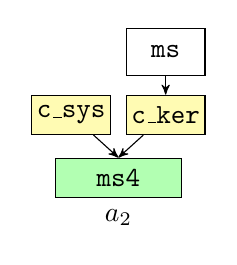
\begin{tikzpicture}[->,>=stealth']

    \node[rectangle,
          draw,
          fill = green!30,
          minimum width = 1.6cm, 
          minimum height = 0.5cm
          ] (ms4) at (0,0) {};
    \node[] at (ms4.center) {\texttt{ms4}};

    \node[rectangle,
    minimum width = 1cm, 
    minimum height = 0.5cm
    ] (lab) at (0,-.5) {};
  \node[] at (lab.center) {$a_2$};

    \node[rectangle,
        draw,
        fill = yellow!30,
        minimum width = 1cm, 
        minimum height = 0.5cm
        ] (sys) at (-.6,.8) {};
    \node[] at (sys.center) {\texttt{c\_sys}};

    \node[rectangle,
        draw,
        fill = yellow!30,
        minimum width = 1cm, 
        minimum height = 0.5cm
        ] (vc) at (.6,.8) {};
    \node[] at (vc.center) {\texttt{c\_ker}};

    \node[rectangle,
        draw,
        minimum width = 1cm, 
        minimum height = 0.6cm
        ] (ms3) at (.6,1.6) {};
    \node[] at (ms3.center) {\texttt{ms}};

%     \node[rectangle,
%     minimum width = 1cm, 
%     minimum height = 0.5cm
%     ] (label) at (0,-0.5) {};
% \node[] at (label.center) {m2b};


    \path[every node/.style={font=\sffamily\small}]
    %host1 path
    (ms3) edge [] node [right] {} (vc.north)
    (vc) edge [] node [right] {} (ms4.north) 
    (sys) edge [] node [right] {} (ms4.north) ;


\end{tikzpicture} & 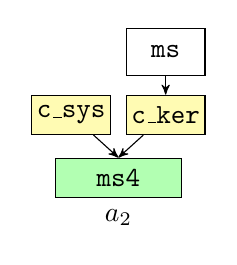
\begin{tikzpicture}[->,>=stealth']

    \node[rectangle,
          draw,
          fill = green!30,
          minimum width = 1.6cm, 
          minimum height = 0.5cm
          ] (ms4) at (0,0) {};
    \node[] at (ms4.center) {\texttt{ms4}};

    \node[rectangle,
    minimum width = 1cm, 
    minimum height = 0.5cm
    ] (lab) at (0,-.5) {};
  \node[] at (lab.center) {$a_2$};

    \node[rectangle,
        draw,
        fill = yellow!30,
        minimum width = 1cm, 
        minimum height = 0.5cm
        ] (sys) at (-.6,.8) {};
    \node[] at (sys.center) {\texttt{c\_sys}};

    \node[rectangle,
        draw,
        fill = yellow!30,
        minimum width = 1cm, 
        minimum height = 0.5cm
        ] (vc) at (.6,.8) {};
    \node[] at (vc.center) {\texttt{c\_ker}};

    \node[rectangle,
        draw,
        minimum width = 1cm, 
        minimum height = 0.6cm
        ] (ms3) at (.6,1.6) {};
    \node[] at (ms3.center) {\texttt{ms}};

%     \node[rectangle,
%     minimum width = 1cm, 
%     minimum height = 0.5cm
%     ] (label) at (0,-0.5) {};
% \node[] at (label.center) {m2b};


    \path[every node/.style={font=\sffamily\small}]
    %host1 path
    (ms3) edge [] node [right] {} (vc.north)
    (vc) edge [] node [right] {} (ms4.north) 
    (sys) edge [] node [right] {} (ms4.north) ;


\end{tikzpicture}  \\   
%                 m2a & m2b & m2c \\ 
%                 &&\\
%                 & \input{examples/ker_vs-sys-seq_reduced/m3.tex}  & \input{examples/rtm_ker-vc-sys-seq_reduced/m3.tex} \\  
%                   & m3b & m3c \\ 
%                  &&\\ 
%                   & 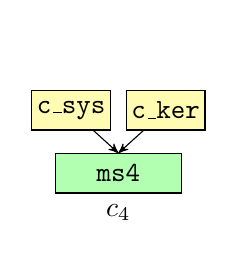
\begin{tikzpicture}[->,>=stealth']

  \node[rectangle,
        draw,
        fill = green!30,
        minimum width = 1.6cm, 
        minimum height = 0.5cm
        ] (ms4) at (0,0) {};
  \node[] at (ms4.center) {\texttt{ms4}};

  \node[rectangle,
  minimum width = 1cm, 
  minimum height = 0.5cm
  ] (lab) at (0,-.5) {};
\node[] at (lab.center) {$c_4$};

  %\node[rectangle,
  %    draw,
  %    minimum width = 1.5cm, 
  %    minimum height = 0.5cm
  %    ] (ms) at (-1,1) {};
  %\node[] at (ms.center) {ms};

  \node[rectangle,
      draw,
      fill = yellow!30,
      minimum width = 1cm, 
      minimum height = 0.5cm
      ] (ker) at (.6,.8) {};
  \node[] at (ker.center) {\texttt{c\_ker}};

  \node[rectangle,
      draw,
      fill = yellow!30,
      minimum width = 1cm, 
      minimum height = 0.5cm
      ] (sys) at (-.6,.8) {};
  \node[] at (sys.center) {\texttt{c\_sys}};

  \node[rectangle,
      minimum width = 1cm, 
      minimum height = 0.5cm
      ] (ms3) at (.6,1.6) {};
  \node[] at (ms3.center) {};

%     \node[rectangle,
%     minimum width = 1cm, 
%     minimum height = 0.5cm
%     ] (label) at (0,-0.5) {};
% \node[] at (label.center) {m3b};


  \path[every node/.style={font=\sffamily\small}]
  %host1 path
  (ker) edge [] node [right] {} (ms4.north)
  (sys) edge [] node [right] {} (ms4.north) ;
  % (ms) edge [] node [right] {} (ms4.north) ;


\end{tikzpicture} & 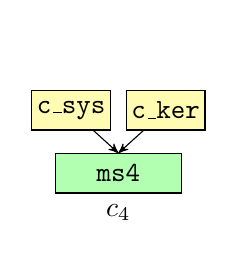
\begin{tikzpicture}[->,>=stealth']

  \node[rectangle,
        draw,
        fill = green!30,
        minimum width = 1.6cm, 
        minimum height = 0.5cm
        ] (ms4) at (0,0) {};
  \node[] at (ms4.center) {\texttt{ms4}};

  \node[rectangle,
  minimum width = 1cm, 
  minimum height = 0.5cm
  ] (lab) at (0,-.5) {};
\node[] at (lab.center) {$c_4$};

  %\node[rectangle,
  %    draw,
  %    minimum width = 1.5cm, 
  %    minimum height = 0.5cm
  %    ] (ms) at (-1,1) {};
  %\node[] at (ms.center) {ms};

  \node[rectangle,
      draw,
      fill = yellow!30,
      minimum width = 1cm, 
      minimum height = 0.5cm
      ] (ker) at (.6,.8) {};
  \node[] at (ker.center) {\texttt{c\_ker}};

  \node[rectangle,
      draw,
      fill = yellow!30,
      minimum width = 1cm, 
      minimum height = 0.5cm
      ] (sys) at (-.6,.8) {};
  \node[] at (sys.center) {\texttt{c\_sys}};

  \node[rectangle,
      minimum width = 1cm, 
      minimum height = 0.5cm
      ] (ms3) at (.6,1.6) {};
  \node[] at (ms3.center) {};

%     \node[rectangle,
%     minimum width = 1cm, 
%     minimum height = 0.5cm
%     ] (label) at (0,-0.5) {};
% \node[] at (label.center) {m3b};


  \path[every node/.style={font=\sffamily\small}]
  %host1 path
  (ker) edge [] node [right] {} (ms4.north)
  (sys) edge [] node [right] {} (ms4.north) ;
  % (ms) edge [] node [right] {} (ms4.north) ;


\end{tikzpicture}  \\
%                  & m4b & m4c \\ 
%                 &&\\  
%                  & 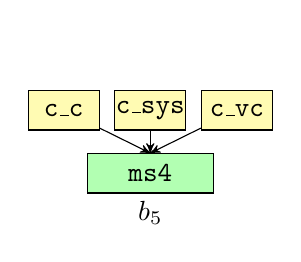
\begin{tikzpicture}[->,>=stealth']

    \node[rectangle,
          draw,
          fill = green!30,
          minimum width = 1.6cm, 
          minimum height = 0.5cm
          ] (ms4) at (0,0) {};
    \node[] at (ms4.center) {\texttt{ms4}};

    \node[rectangle,
    minimum width = 1cm, 
    minimum height = 0.5cm
    ] (lab) at (0,-.5) {};
  \node[] at (lab.center) {$b_5$};

    \node[rectangle,
        draw,
        fill = yellow!30,
        minimum width = .9cm, 
        minimum height = 0.5cm
        ] (vc) at (1.1,.8) {};
    \node[] at (vc.center) {\texttt{c\_vc}};

    \node[rectangle,
        draw,
        fill = yellow!30,
        minimum width = .9cm, 
        minimum height = 0.5cm
        ] (c) at (-1.1,.8) {};
    \node[] at (c.center) {\texttt{c\_c}};

    \node[rectangle,
        draw,
        fill = yellow!30,
        minimum width = .9cm, 
        minimum height = 0.5cm
        ] (sys) at (0,.8) {};
    \node[] at (sys.center) {\texttt{c\_sys}};

    \node[rectangle,
        minimum width = .9cm, 
        minimum height = 0.5cm
        ] (ms3) at (1.1,1.6) {};
    \node[] at (ms3.center) {};


    \path[every node/.style={font=\sffamily\small}]
    %host1 path
    (vc) edge [] node [right] {} (ms4.north)
    (c) edge [] node [right] {} (ms4.north)
    (sys) edge [] node [right] {} (ms4.north) ;
    % (ms) edge [] node [right] {} (ms4.north) ;


\end{tikzpicture} & 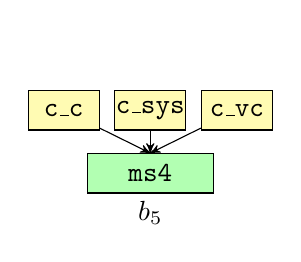
\begin{tikzpicture}[->,>=stealth']

    \node[rectangle,
          draw,
          fill = green!30,
          minimum width = 1.6cm, 
          minimum height = 0.5cm
          ] (ms4) at (0,0) {};
    \node[] at (ms4.center) {\texttt{ms4}};

    \node[rectangle,
    minimum width = 1cm, 
    minimum height = 0.5cm
    ] (lab) at (0,-.5) {};
  \node[] at (lab.center) {$b_5$};

    \node[rectangle,
        draw,
        fill = yellow!30,
        minimum width = .9cm, 
        minimum height = 0.5cm
        ] (vc) at (1.1,.8) {};
    \node[] at (vc.center) {\texttt{c\_vc}};

    \node[rectangle,
        draw,
        fill = yellow!30,
        minimum width = .9cm, 
        minimum height = 0.5cm
        ] (c) at (-1.1,.8) {};
    \node[] at (c.center) {\texttt{c\_c}};

    \node[rectangle,
        draw,
        fill = yellow!30,
        minimum width = .9cm, 
        minimum height = 0.5cm
        ] (sys) at (0,.8) {};
    \node[] at (sys.center) {\texttt{c\_sys}};

    \node[rectangle,
        minimum width = .9cm, 
        minimum height = 0.5cm
        ] (ms3) at (1.1,1.6) {};
    \node[] at (ms3.center) {};


    \path[every node/.style={font=\sffamily\small}]
    %host1 path
    (vc) edge [] node [right] {} (ms4.north)
    (c) edge [] node [right] {} (ms4.north)
    (sys) edge [] node [right] {} (ms4.north) ;
    % (ms) edge [] node [right] {} (ms4.north) ;


\end{tikzpicture}   \\
%                  & m5b & m5c \\ 
%                 &&\\
%             \end{tabular}
%     \end{center}
%     \caption{Reduced attack graphs for sys, ker-vc-sys-seq, and rtm-ker-vc-sys-seq}
%     \label{fig:rtm-compare-reduced}
% \end{figure}

% Employing the previously introduced formalism, it becomes possible to demonstrate that \emph{rtm-ker-vc-sys-seq} is indeed the most resistant to attacks, establishing it as the optimal protocol. 

Formal reasoning to demonstrate that \emph{rtm-ker-vc-sys-seq} is indeed the most resistant to attacks begins by obtaining the Chase generated attack graphs for each protocol. With the protocols presented in Table \ref{Chase-table} and the necessary Chase inputs, we obtain the following attack models presented in Figure \ref{fig:rtm-compare}. After applying graph normalization, the attack graphs can be reduced to only activities that affect an active adversary, as presented in Figure \ref{fig:rtm-compare-reduced}.  The remainder of this analysis will only consider the graphs under normal form. 

\newpage

Employing the previously introduced formalism to determine the relationship between the three protocols begins by analyzing the underlying relationship between individual attack graphs. Starting with \texttt{m1a}, it is apparent that \texttt{m1b} is strictly better than \texttt{m1a} because \texttt{m1b} has a time-constrained measurement event. The same logic applies when comparing \texttt{m2a} and \texttt{m2b}. It is also apparent that graph \texttt{m3b} is equivalent to \texttt{m2a} because they have the same corruption events. \texttt{m4b} is strictly better than either \texttt{m2a} or \texttt{m1a} because it has more corruption events. By the same reasoning, \texttt{m5b} is strictly better than \texttt{m1a}. This concludes comparison of the individual attack graphs.

Next, we apply the supports formalism to determine the relationship between the sets of attack graphs. Because every graph generated by \texttt{ker-vc-sys-seq} requires the adversary to apply either the same effort or more effort to attack when compared to \texttt{sys}, we say that \texttt{ker-vc-sys-seq} is at least as adversary constrained as \texttt{sys}. Said differently, we find that \texttt{ker-vc-sys-seq} supports \texttt{sys}, as denoted with the following relation: 

\begin{center}
    sys $\leq$ ker-vs-sys-seq
\end{center}

We apply the same logic to compare \texttt{ker-vc-sys-seq} and \texttt{rtm-ker-vc-sys-seq}. That is, we first compare the protocols' individual Chase-generated attack graphs. Again, looking at the reduced graphs in Figure \ref{fig:rtm-compare-reduced}, we see that  \texttt{m1c} and  \texttt{m1b} are the same graph; they are equivalent under the bidirectional homomorphism. \texttt{m2c} and \texttt{m2b} are also the same graph thus equivalent. \texttt{m3c} has more time-constrained corruption events when compared to  \texttt{m3b} thus  \texttt{m3c} is strictly better than \texttt{m3b}. The same logic applies to \texttt{m4c} and  \texttt{m4b} where  \texttt{m4b} is strictly less than  \texttt{m4c} because  \texttt{m4c} has more time-constrained corruption events.  \texttt{m5c} and \texttt{m5b} are equivalent. Propagating the findings of individual attack graph comparisons and considering the formalism of supports, we conclude that \texttt{ker-vc-sys-seq} is less than or equal to \texttt{rtm-ker-vc-sys-seq} because every graph in \texttt{rtm-ker-vc-sys-seq} requires the adversary to perform equal or more effort to attack when compared to every graph in  \texttt{ker-vc-sys-seq}. 

Ultimately, we arrive at the ordering below. Formal analysis therefore supports our hypothesis that a measurement which considers system dependencies up to a root of trust, is more difficult to attack and therefore better constrains the adversary. 
\begin{center}
    sys $\leq$ ker-vc-sys-seq $\leq$ rtm-ker-vc-sys-seq
\end{center}

%% next example is measuring from a different place 
Secondly, we investigate the impact of measurement location on adversary constraint specifically studying the effects of attacks when all measurements are carried out on the same platform compared to a separate platform. To test this hypothesis, the following protocols presented in Table \ref{Chase-table-location} were analyzed with Chase and subsequently subjected to the ordering methodology. The baseline protocol \texttt{sys} calls the virus checker located on \texttt{p4} to measure the system \texttt{sys}. The next protocol \texttt{ker-vc-sys-seq} calls the kernel ASP \emph{ker} to measure the virus checker $vc$ prior to the \texttt{sys} measurement. It is important to note that the kernel ASP is located on the same platform, $P4$, as \emph{vc} and \emph{sys}. Again, we know from the system description, that the system depends on the virus checker and the virus checker depends on the kernel. In the third protocol, \texttt{a1-vc-sys-seq}, the ASP \emph{a1}, located on a separate platform \emph{p3}, is used to measure the virus checker prior to the \texttt{sys} measurement. \emph{a1} is not included in the dependency chain of \emph{vc} or \emph{sys} but simply another attestation capability within the target system.

% \begin{table}[htbp]
%     \setlength\extrarowheight{7pt}
%     \centering
%     \begin{tabular}{|M{4cm}|M{10cm}|N}
%     \hline
%         Protocol Name & Actual protocol &\\
%     \hline
%         sys & *target: $\at{p4}{(vc\; p4\; sys)}$  &\\ 
%     \hline   
%         ker-vc-sys-seq & *target:  $\at{p4}{[(ker\; p4\; vc)}$ \texttt{+<+} $\at{p4}{(vc\; p4\; sys)}]$ &\\ 
%     \hline
%      a1-vc-sys-seq & *target: $\at{p3}{[(a1\; p4\; vc)}$ \texttt{+<+} $\at{p4}{(vc\; p4\; sys)}]$ &\\ \hline 
%     \end{tabular}
%     \caption[Chase Analysis with Varied Place]{Protocols analyzed regarding location of prior measurements with Chase}
%     \label{Chase-table-location}
% \end{table}

% \begin{figure}[hbtp]
%     %\setlength\extrarowheight{20pt}
%     \begin{center}
%         % \begin{tabular}{ M{3.75cm} | M{5cm} | M{5cm}}
%         \begin{tabular}{ c | c | c}
%         sys & ker-vc-sys-seq & a1-vc-sys-seq \\
%         \hline
%         &&\\
%         \input{examples/sys/sys1.tex} & \input{examples/ker_vs-sys-seq_reduced/m1.tex} & \input{examples/a1-vc-sys-seq/vc-sys-seq1.tex}  \\ 
%         m1a & m1b & m1c \\ 
%         &&\\
%         \begin{tikzpicture}[->,>=stealth']

    \node[rectangle,
          draw,
          fill = green!30,
          minimum width = 2cm, 
          minimum height = 0.5cm
          ] (ms4) at (0,0) {};
    \node[] at (ms4.center) {\texttt{ms4}};


    \node[rectangle,
        draw,
        fill = yellow!30,
        minimum width = 1.5cm, 
        minimum height = 0.5cm
        ] (sys) at (-1,1) {};
    \node[] at (sys.center) {\texttt{c\_sys}};

    \node[rectangle,
        draw,
        fill = yellow!30,
        minimum width = 1.5cm, 
        minimum height = 0.5cm
        ] (ker) at (1,1) {};
    \node[] at (ker.center) {\texttt{c\_ker}};

    \node[rectangle,
        minimum width = 1.5cm, 
        minimum height = 0.5cm
        ] (ms3) at (1,2) {};
    \node[] at (ms3.center) {};


    % \node[rectangle,
    %     minimum width = 1cm, 
    %     minimum height = 0.5cm
    %     ] (label) at (0,-1) {};
    % \node[] at (label.center) {m2a};


    \path[every node/.style={font=\sffamily\small}]
    %host1 path
    (vc) edge [] node [right] {} (ms4.north) 
    (sys) edge [] node [right] {} (ms4.north) ;


\end{tikzpicture} & 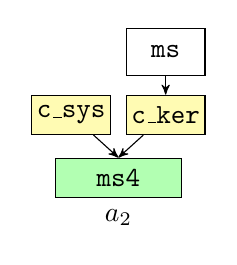
\begin{tikzpicture}[->,>=stealth']

    \node[rectangle,
          draw,
          fill = green!30,
          minimum width = 1.6cm, 
          minimum height = 0.5cm
          ] (ms4) at (0,0) {};
    \node[] at (ms4.center) {\texttt{ms4}};

    \node[rectangle,
    minimum width = 1cm, 
    minimum height = 0.5cm
    ] (lab) at (0,-.5) {};
  \node[] at (lab.center) {$a_2$};

    \node[rectangle,
        draw,
        fill = yellow!30,
        minimum width = 1cm, 
        minimum height = 0.5cm
        ] (sys) at (-.6,.8) {};
    \node[] at (sys.center) {\texttt{c\_sys}};

    \node[rectangle,
        draw,
        fill = yellow!30,
        minimum width = 1cm, 
        minimum height = 0.5cm
        ] (vc) at (.6,.8) {};
    \node[] at (vc.center) {\texttt{c\_ker}};

    \node[rectangle,
        draw,
        minimum width = 1cm, 
        minimum height = 0.6cm
        ] (ms3) at (.6,1.6) {};
    \node[] at (ms3.center) {\texttt{ms}};

%     \node[rectangle,
%     minimum width = 1cm, 
%     minimum height = 0.5cm
%     ] (label) at (0,-0.5) {};
% \node[] at (label.center) {m2b};


    \path[every node/.style={font=\sffamily\small}]
    %host1 path
    (ms3) edge [] node [right] {} (vc.north)
    (vc) edge [] node [right] {} (ms4.north) 
    (sys) edge [] node [right] {} (ms4.north) ;


\end{tikzpicture} & \input{examples/a1-vc-sys-seq/vc-sys-seq2.tex}  \\ 
%         m2a & m2b & m2c \\
%         &&\\    & \input{examples/ker_vs-sys-seq_reduced/m3.tex} & \input{examples/a1-vc-sys-seq/vc-sys-seq3.tex}  \\ 
%             & m3b & m3c \\
%         &&\\  & 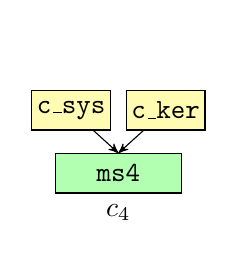
\begin{tikzpicture}[->,>=stealth']

  \node[rectangle,
        draw,
        fill = green!30,
        minimum width = 1.6cm, 
        minimum height = 0.5cm
        ] (ms4) at (0,0) {};
  \node[] at (ms4.center) {\texttt{ms4}};

  \node[rectangle,
  minimum width = 1cm, 
  minimum height = 0.5cm
  ] (lab) at (0,-.5) {};
\node[] at (lab.center) {$c_4$};

  %\node[rectangle,
  %    draw,
  %    minimum width = 1.5cm, 
  %    minimum height = 0.5cm
  %    ] (ms) at (-1,1) {};
  %\node[] at (ms.center) {ms};

  \node[rectangle,
      draw,
      fill = yellow!30,
      minimum width = 1cm, 
      minimum height = 0.5cm
      ] (ker) at (.6,.8) {};
  \node[] at (ker.center) {\texttt{c\_ker}};

  \node[rectangle,
      draw,
      fill = yellow!30,
      minimum width = 1cm, 
      minimum height = 0.5cm
      ] (sys) at (-.6,.8) {};
  \node[] at (sys.center) {\texttt{c\_sys}};

  \node[rectangle,
      minimum width = 1cm, 
      minimum height = 0.5cm
      ] (ms3) at (.6,1.6) {};
  \node[] at (ms3.center) {};

%     \node[rectangle,
%     minimum width = 1cm, 
%     minimum height = 0.5cm
%     ] (label) at (0,-0.5) {};
% \node[] at (label.center) {m3b};


  \path[every node/.style={font=\sffamily\small}]
  %host1 path
  (ker) edge [] node [right] {} (ms4.north)
  (sys) edge [] node [right] {} (ms4.north) ;
  % (ms) edge [] node [right] {} (ms4.north) ;


\end{tikzpicture} & \input{examples/a1-vc-sys-seq/vc-sys-seq4.tex}  \\ 
%         & m4b & m4c \\
%         &&\\ & 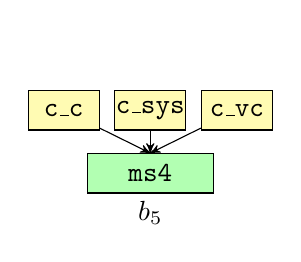
\begin{tikzpicture}[->,>=stealth']

    \node[rectangle,
          draw,
          fill = green!30,
          minimum width = 1.6cm, 
          minimum height = 0.5cm
          ] (ms4) at (0,0) {};
    \node[] at (ms4.center) {\texttt{ms4}};

    \node[rectangle,
    minimum width = 1cm, 
    minimum height = 0.5cm
    ] (lab) at (0,-.5) {};
  \node[] at (lab.center) {$b_5$};

    \node[rectangle,
        draw,
        fill = yellow!30,
        minimum width = .9cm, 
        minimum height = 0.5cm
        ] (vc) at (1.1,.8) {};
    \node[] at (vc.center) {\texttt{c\_vc}};

    \node[rectangle,
        draw,
        fill = yellow!30,
        minimum width = .9cm, 
        minimum height = 0.5cm
        ] (c) at (-1.1,.8) {};
    \node[] at (c.center) {\texttt{c\_c}};

    \node[rectangle,
        draw,
        fill = yellow!30,
        minimum width = .9cm, 
        minimum height = 0.5cm
        ] (sys) at (0,.8) {};
    \node[] at (sys.center) {\texttt{c\_sys}};

    \node[rectangle,
        minimum width = .9cm, 
        minimum height = 0.5cm
        ] (ms3) at (1.1,1.6) {};
    \node[] at (ms3.center) {};


    \path[every node/.style={font=\sffamily\small}]
    %host1 path
    (vc) edge [] node [right] {} (ms4.north)
    (c) edge [] node [right] {} (ms4.north)
    (sys) edge [] node [right] {} (ms4.north) ;
    % (ms) edge [] node [right] {} (ms4.north) ;


\end{tikzpicture} & \\
%         & m5b &  \\
%         \end{tabular}
%     \end{center}
%     \caption{Reduced attack graphs for sys, ker-vc-sys-seq, and a1-vc-sys-seq}
%     \label{fig:chase-location}
% \end{figure}

One may hypothesize that \texttt{ker-vc-sys-seq} is the strongest measurement because it includes measurements within the system's dependency chain. However, the generated Chase models, presented in Figure \ref{fig:chase-location} in their normal form, did not support this hypothesis. When first analyzing the graphs, it is apparent that both protocols \texttt{ker-vc-sys-seq} and \texttt{a1-vc-sys-seq} are at least as good as \texttt{sys}. This claim holds because all attack graphs in the more detailed protocols are the same or require more effort than the attack graphs generated by \texttt{sys}. However, when comparing \texttt{ker-vc-sys-seq} and \texttt{a1-vc-sys-seq} the relationship is harder to recognize. For instance, consider the graph \texttt{m4b}. It is more difficult to attack when compared to \texttt{m1a} or \texttt{m2a} because it has more corruption events. However, there is not a relatable graph in \texttt{a1-vc-sys-seq} because there is no graph that includes corruption events of \emph{vc}, \emph{ker}, and \emph{sys}. A similar Chase generated model may be \texttt{m3c} or \texttt{m4c}, but adversary events do not have the same label. Therefore, we must conclude that  \texttt{ker-vc-sys-seq} and \texttt{a1-vc-sys-seq} are incomparable. This may actually be desired behavior because we cannot make claims about the difficulty of a specific attack. 


%% third example for ordering 
The third facet of protocol ordering investigates the impact of Copland protocol composition, sequential versus parallel, on adversary capability. \citet{Rowe:2021:AutomatedTrust} motivates the use of Chase to compare attack difficultly, manually studying specific examples with sequential measurements that mimic the system's dependency structure versus parallel measurements with no specified order. \citet{Rowe:2021:AutomatedTrust} logically deduced sequential measurements would better constrain the adversary because measuring within the system's dependency structure would require more complex attacks. We set out to apply our mathematical model to this hypothesis, testing the effects of protocol composition over the target system in Figure \ref{fig:ord-system}. 

In Table \ref{Chase-table-order}, we present three protocols where the latter two have varied composition. The first protocol, \texttt{sys}, is a baseline measurement. The next two protocols include an additional measurement involving the kernel $ker$ measuring the virus checker $vc$. The difference between the two measurements is the composition. In \texttt{ker-vc-sys-seq}, the measurements are performed in sequence. In \texttt{ker-vc-sys-par}, measurements are performed in parallel. By altering the composition dynamics in these protocols, we are able to investigate the effects on adversary constraint.

% \begin{table}[htbp]
%     \setlength\extrarowheight{7pt}
%     \centering
%     \begin{tabular}{|M{4cm}|M{10cm}|N}
%     \hline
%         Protocol Name & Actual protocol &\\
%     \hline
%         sys & *target: $\at{p4}{(vc\; p4\; sys)}$  &\\ 
%     \hline
%     ker-vc-sys-seq & *target:  $\at{p4}{[(ker\; p4\; vc)}$ \texttt{+<+} $\at{p4}{(vc\; p4\; sys)}]$ &\\ \hline 
%     ker-vc-sys-par & *target: $\at{p3}{[(ker\; p4\; vc)}$ \texttt{+}$\sim$\texttt{+} $\at{p4}{(vc\; p4\; sys)}]$ &\\ 
%         \hline   
%     \end{tabular}
%     \caption[Chase Analysis with Varied Composition]{Protocols analyzed regarding measurement composition with Chase}
%     \label{Chase-table-order}
% \end{table}

%Beyond the protocol input incorporating diverse composition operators, we maintain consistency in utilizing identical files for the Chase input to ensure accurate analysis. 
Executing Chase with the three distinct protocols yields the normalized attack graphs presented in Figure \ref{fig:chase-comp-graphs} where protocol ordering methodology yields incomparable results between the sequential and parallel protocols. Upon analyzing these graphs, it becomes evident that the inclusion of additional measurement operations -- specifically those mirroring the dependency chain -- more effectively constrains an adversary. This observation arises from the comparison of \texttt{sys} with both \texttt{ker-vc-sys-seq} and \texttt{ker-vc-sys-par}, wherein both of the latter protocols support \texttt{sys}. When evaluating the relationship between \texttt{ker-vc-sys-seq} and \texttt{ker-vc-sys-par}, determining which one supports the other is not obvious. Notably, graphs \texttt{m2b} and \texttt{m2c} are identical and therefore equal. Similarly, \texttt{m1c} and \texttt{m3b} involve the same attacks and culminate in the same final measurement event, so they are equivalent. The complexity arises when comparing \texttt{m3c} to other attack graphs. While \texttt{m3c} is more difficult to attack than \texttt{m2a} due to the additional adversary (repair) event, comparing it with any graph generated by \texttt{ker-vc-sys-par} in its current form is impossible. Since the final measurement event of \texttt{m3c} differs from that in any graph generated by \texttt{ker-vc-sys-par} and the repair event cannot be found in any graph generated by \texttt{ker-vc-sys-par}, we find that \texttt{ker-vc-sys-seq} and \texttt{ker-vc-sys-par} are incomparable. This contradicts the conclusions presented by \citet{Rowe:2021:AutomatedTrust}. 

% \begin{figure}
% \begin{center}
% \begin{tabular}{ c |  c | c }
%     sys & ker-vc-sys-seq & ker-vc-sys-par  \\
%     \hline
%     &&\\
%     \input{examples/sys/sys1.tex} & \input{examples/ker_vs-sys-seq_reduced/m1.tex} & \input{examples/vc-sys-par/m1'.tex} \\
%     m1a & m1b & m1c \\ 
%     &&\\
%     \begin{tikzpicture}[->,>=stealth']

    \node[rectangle,
          draw,
          fill = green!30,
          minimum width = 2cm, 
          minimum height = 0.5cm
          ] (ms4) at (0,0) {};
    \node[] at (ms4.center) {\texttt{ms4}};


    \node[rectangle,
        draw,
        fill = yellow!30,
        minimum width = 1.5cm, 
        minimum height = 0.5cm
        ] (sys) at (-1,1) {};
    \node[] at (sys.center) {\texttt{c\_sys}};

    \node[rectangle,
        draw,
        fill = yellow!30,
        minimum width = 1.5cm, 
        minimum height = 0.5cm
        ] (ker) at (1,1) {};
    \node[] at (ker.center) {\texttt{c\_ker}};

    \node[rectangle,
        minimum width = 1.5cm, 
        minimum height = 0.5cm
        ] (ms3) at (1,2) {};
    \node[] at (ms3.center) {};


    % \node[rectangle,
    %     minimum width = 1cm, 
    %     minimum height = 0.5cm
    %     ] (label) at (0,-1) {};
    % \node[] at (label.center) {m2a};


    \path[every node/.style={font=\sffamily\small}]
    %host1 path
    (vc) edge [] node [right] {} (ms4.north) 
    (sys) edge [] node [right] {} (ms4.north) ;


\end{tikzpicture} & 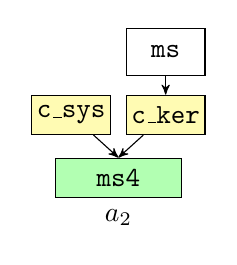
\begin{tikzpicture}[->,>=stealth']

    \node[rectangle,
          draw,
          fill = green!30,
          minimum width = 1.6cm, 
          minimum height = 0.5cm
          ] (ms4) at (0,0) {};
    \node[] at (ms4.center) {\texttt{ms4}};

    \node[rectangle,
    minimum width = 1cm, 
    minimum height = 0.5cm
    ] (lab) at (0,-.5) {};
  \node[] at (lab.center) {$a_2$};

    \node[rectangle,
        draw,
        fill = yellow!30,
        minimum width = 1cm, 
        minimum height = 0.5cm
        ] (sys) at (-.6,.8) {};
    \node[] at (sys.center) {\texttt{c\_sys}};

    \node[rectangle,
        draw,
        fill = yellow!30,
        minimum width = 1cm, 
        minimum height = 0.5cm
        ] (vc) at (.6,.8) {};
    \node[] at (vc.center) {\texttt{c\_ker}};

    \node[rectangle,
        draw,
        minimum width = 1cm, 
        minimum height = 0.6cm
        ] (ms3) at (.6,1.6) {};
    \node[] at (ms3.center) {\texttt{ms}};

%     \node[rectangle,
%     minimum width = 1cm, 
%     minimum height = 0.5cm
%     ] (label) at (0,-0.5) {};
% \node[] at (label.center) {m2b};


    \path[every node/.style={font=\sffamily\small}]
    %host1 path
    (ms3) edge [] node [right] {} (vc.north)
    (vc) edge [] node [right] {} (ms4.north) 
    (sys) edge [] node [right] {} (ms4.north) ;


\end{tikzpicture} & \input{examples/vc-sys-par/m2'.tex} \\
%     m2a & m2b & m2c \\ 
%     &&\\
%     & \input{examples/ker_vs-sys-seq_reduced/m3.tex} & \input{examples/vc-sys-par/m3'.tex} \\ 
%     & m3b & m3c \\ 
%     &&\\
%     & 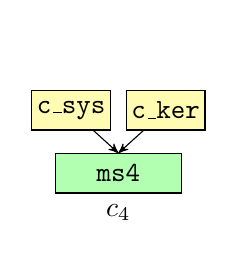
\begin{tikzpicture}[->,>=stealth']

  \node[rectangle,
        draw,
        fill = green!30,
        minimum width = 1.6cm, 
        minimum height = 0.5cm
        ] (ms4) at (0,0) {};
  \node[] at (ms4.center) {\texttt{ms4}};

  \node[rectangle,
  minimum width = 1cm, 
  minimum height = 0.5cm
  ] (lab) at (0,-.5) {};
\node[] at (lab.center) {$c_4$};

  %\node[rectangle,
  %    draw,
  %    minimum width = 1.5cm, 
  %    minimum height = 0.5cm
  %    ] (ms) at (-1,1) {};
  %\node[] at (ms.center) {ms};

  \node[rectangle,
      draw,
      fill = yellow!30,
      minimum width = 1cm, 
      minimum height = 0.5cm
      ] (ker) at (.6,.8) {};
  \node[] at (ker.center) {\texttt{c\_ker}};

  \node[rectangle,
      draw,
      fill = yellow!30,
      minimum width = 1cm, 
      minimum height = 0.5cm
      ] (sys) at (-.6,.8) {};
  \node[] at (sys.center) {\texttt{c\_sys}};

  \node[rectangle,
      minimum width = 1cm, 
      minimum height = 0.5cm
      ] (ms3) at (.6,1.6) {};
  \node[] at (ms3.center) {};

%     \node[rectangle,
%     minimum width = 1cm, 
%     minimum height = 0.5cm
%     ] (label) at (0,-0.5) {};
% \node[] at (label.center) {m3b};


  \path[every node/.style={font=\sffamily\small}]
  %host1 path
  (ker) edge [] node [right] {} (ms4.north)
  (sys) edge [] node [right] {} (ms4.north) ;
  % (ms) edge [] node [right] {} (ms4.north) ;


\end{tikzpicture} &  \\
%     & m4b & \\ 
%     &&\\    
% \end{tabular}
% \end{center}
% \caption{Reduced attack graphs for \texttt{ker-vc-sys-seq} and \texttt{ker-vc-sys-par}}
% \label{fig:chase-comp-graphs}
% \end{figure}

An intriguing nuance emerging from studying protocol compositions is the frequent occurrence of attack graphs with repair events in the Chase output of Copland phrases with parallel measurement operations. It is common to find instances where parallel measurements, mimicking the dependency chain, are not executed in an order that replicates the dependencies. Consequently, the Chase analysis often includes graphs where, at the top level measurement, the adversary corrupts a component but then must subsequently repair it before it undergoes measurement. This scenario precisely unfolds in graph m3c: the virus checker is corrupted, leading to a measurement of a compromised system, but repair becomes necessary before the virus checker itself is measured.

This observation prompts us to consider the effort involved in a repair event. That is, if an adversary already has a foothold in the system through a previously corrupted component, how challenging is it for them to repair that same component? The difficulty of this decision is context-dependent and lies within the judgment of an informed analyst. If informed attestation analyst determines that the effort required for the repair event in graph \texttt{m3c} is minimal, then perhaps graph \texttt{m3c} is equivalent to graph \texttt{m2a} or strictly less than graph \texttt{m2a}. Following this order, \texttt{ker-vc-sys-seq} supports both \texttt{ker-vc-sys-par} and \texttt{sys}, leading us to conclude that \texttt{ker-vc-sys-seq} is the most difficult to attack and therefore the best protocol. This conclusion would align with the intuition presented by \citet{Rowe:2021:AutomatedTrust}.

%\subsubsection*{Summary}

These examples demonstrate the applicability of this ordering approach to examples from the literature. With these completed examples, we reliably conclude our adversary-constrained protocol ordering methodology successfully enhances the evaluation of remote attestation protocols. Leveraging the Chase model finder, we order Copland protocols according to their adversary constraint by comparing all possible attack graphs and linking the relationship between attack graphs to the protocol in question. By testing various protocol composition and protocol ordering hypotheses regarding Copland phrases, we reliably conclude that measuring according to the system's dependency chain provably increases the trustworthiness of generated evidence. This methodology introduces a novel approach to protocol ordering, paving the way for more complex examples to ultimately create more robust and resilient attestation systems.


\section*{Appendix}


%%%%%%%%%%%
% Quick and dirty example using \verb+listings+ to format Coq code:

% \begin{lstlisting}[language=coq]
%   Definition x:nat := 3.
%   Fixpoint f(x:nat):nat := if x=0 then 1 else x*f(x-1).
% \end{lstlisting}

%
% 
% ---- Bibliography ----
%
% BibTeX users should specify bibliography style 'splncs04'.
% References will then be sorted and formatted in the correct style.
%
%\bibliographystyle{splncs04}
\bibliographystyle{splncsnat}
%\bibliography{sldg}
\bibliography{works}
%
\end{document}
